\section*{Introduction}\index{Antliophora}
\textbf{Mecoptera}, \textbf{Siphonaptera}, and \textbf{Diptera} together comprise a lineage called \textbf{Antliophora} (Gr. for ``pump bearers''), insects characterized by the presence of a sperm pump. Diptera is one of the ``big four'' orders of insects, and with \textgreater154,000 described species (15\% of the total estimated diversity) this taxon is a candidate for the most diverse order of insects.

\section{Mecoptera}\index{Mecoptera}
Siphonaptera and Mecoptera exhibit some really interesting phenotypes, such as the presence of elongate acanthae in the proventriculus and a unique, resilin-based jumping mechanism. These orders are undoubtedly closely related, with some phylogenies placing Siphonaptera within Mecoptera, sister to Boreidae or Nannochoristidae. These topologies, however, are not yet a robust, and we treat these insects as separate in lab. Mecoptera exhibit the following characters:
\begin{itemize}
\item fore wing (if present) with \textless4 costal crossveins, 20+ closed cells
\item head prolonged below eyes as a beak or rostrum, with chewing mouthparts at tip
\end{itemize}

\subsubsection{Panorpidae (scorpionflies)}\index{Panorpidae}
\noindent{}\textit{Diagnostic characters:} Tarsi not raptorial, and with two small claws apically; wings fairly broad at base; male genitalia somewhat resemble scorpion sting.\vspace{3mm}

\noindent{}\textit{Natural history:} As adults these insects generally scavenge on dead or nearly dead insects, including prey caught in spider webs. Larvae are likewise scavenger, mostly in leaf litter. There are about 350 species worldwide.

\begin{figure}[ht!]
  \centering
    \includegraphics[width=0.5\textwidth]{antliophora/Panorpidae}
  \caption{Panorpidae \citep[modified from Fig. 60 in][]{bhlitem105840ross}}
  \label{fig:panorpid}
\end{figure}

\subsubsection{Bittacidae (hangingflies)}\index{Bittacidae}
\noindent{}\textit{Diagnostic characters:} Tarsi each with one large claw; tarsi raptorial, tarsomere 5 fold back against tarsomere 4; wings narrower at base; usually crane fly like in appearance, occasionally wingless.\vspace{3mm}

\noindent{}\textit{Natural history:} Hangingflies are predators of other insects. Males usually offer prey to females as nuptial gifts. There are about 170 species worldwide.\vspace{3mm}

\begin{theo}
{}Compare the leg morphology of these insects to Panorpidae. Can you predict how the legs function? What adaptations do you see?
\end{theo}

\begin{figure}[ht!]
  \centering
    \reflectbox{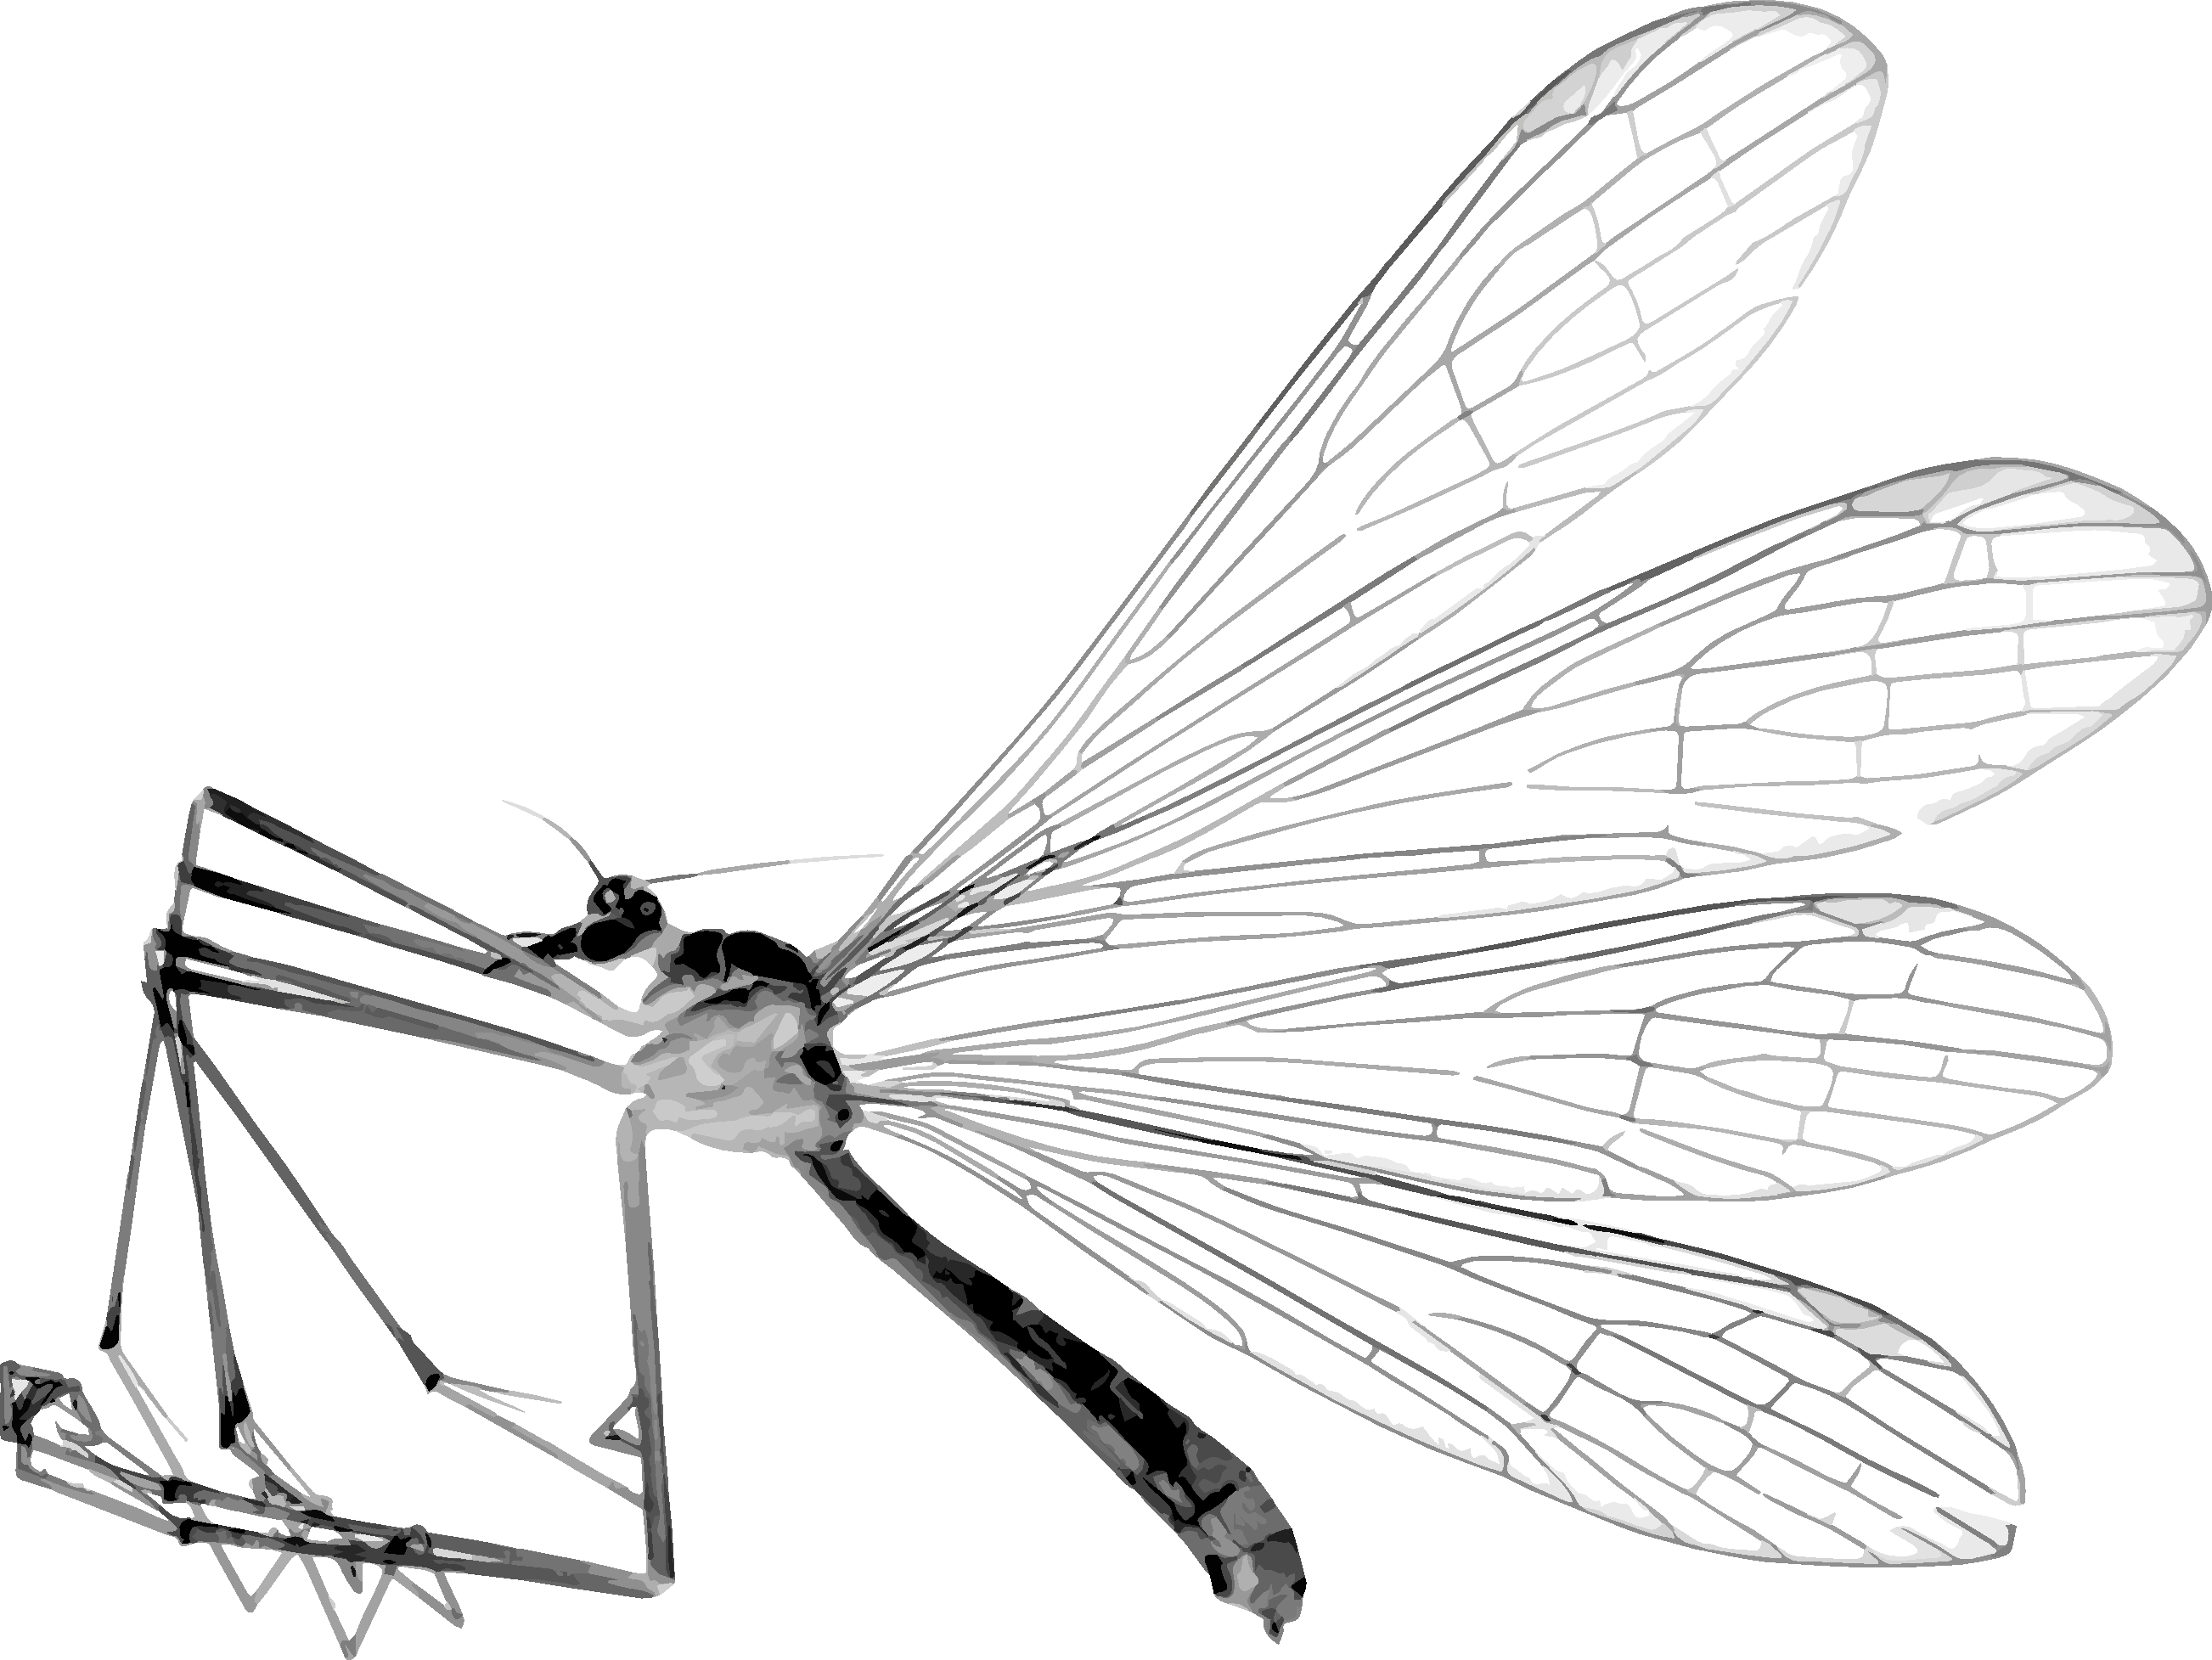
\includegraphics[width=0.5\textwidth]{antliophora/BittacidHabitus}}
  \caption{Bittacidae \citep[Modified from][Fig. 1]{Du_Hua_2017}}
  \label{fig:bittacid}
\end{figure}

\subsubsection{Boreidae (snow scorpionflies)}\index{Boreidae}
\noindent{}\textit{Diagnostic characters:} Body usually mostly brown or black; antennae long; wings vestigial and hind legs long, saltatorial (may not be obvious unless you examine internal characters); female has a straight ovipositor about the same length as the rostrum; males have a blunt, rounded abdominal tip.\vspace{3mm}

\noindent{}\textit{Natural history:} As the common name suggests, adults of these insects can be found in winter, crawling or standing on snow, often at the bases of trees. Larvae and adults feed on mosses and liverworts. Males use their claw-like wings to hold onto the female. About 30 species have been described worldwide.

\begin{figure}[ht!]
  \centering
    \reflectbox{\includegraphics[width=0.5\textwidth]{antliophora/BoreidHabitus}}
  \caption{Boreidae. Photo (CC BY-SA 4.0 International) by H\aa{}kan S\"oderholm (Wikimedia Commons)}
  \label{fig:boreid}
\end{figure}

\section{Siphonaptera (fleas)}\index{Siphonaptera}
\begin{itemize}
\item usually small, laterally flattened ectoparasites of vertebrates
\item wingless, laterally flattened, spiny
\item antennae small, set back in grooves (scrobes) on the head
\item eyes reduced in size
\item legs adapted in part for jumping
\end{itemize}

\begin{theo}
{}Given the above characters and others you observe on the specimens we have in lab, describe three adaptations to living and feeding on a vertebrate host.
\end{theo}

\subsubsection{Pulicidae (dog, cat fleas)}\index{Pulicidae}
\noindent{}\textit{Diagnostic characters:} Mid coxa without internal ridge; hind tibia without apical tooth.\vspace{3mm}

\noindent{}\textit{Natural history:} This family includes most of the species that bite humans and domestic animals. At least one pulicid vectors plague. The family includes about 170 species worldwide.

\begin{figure}[ht!]
  \centering
    \reflectbox{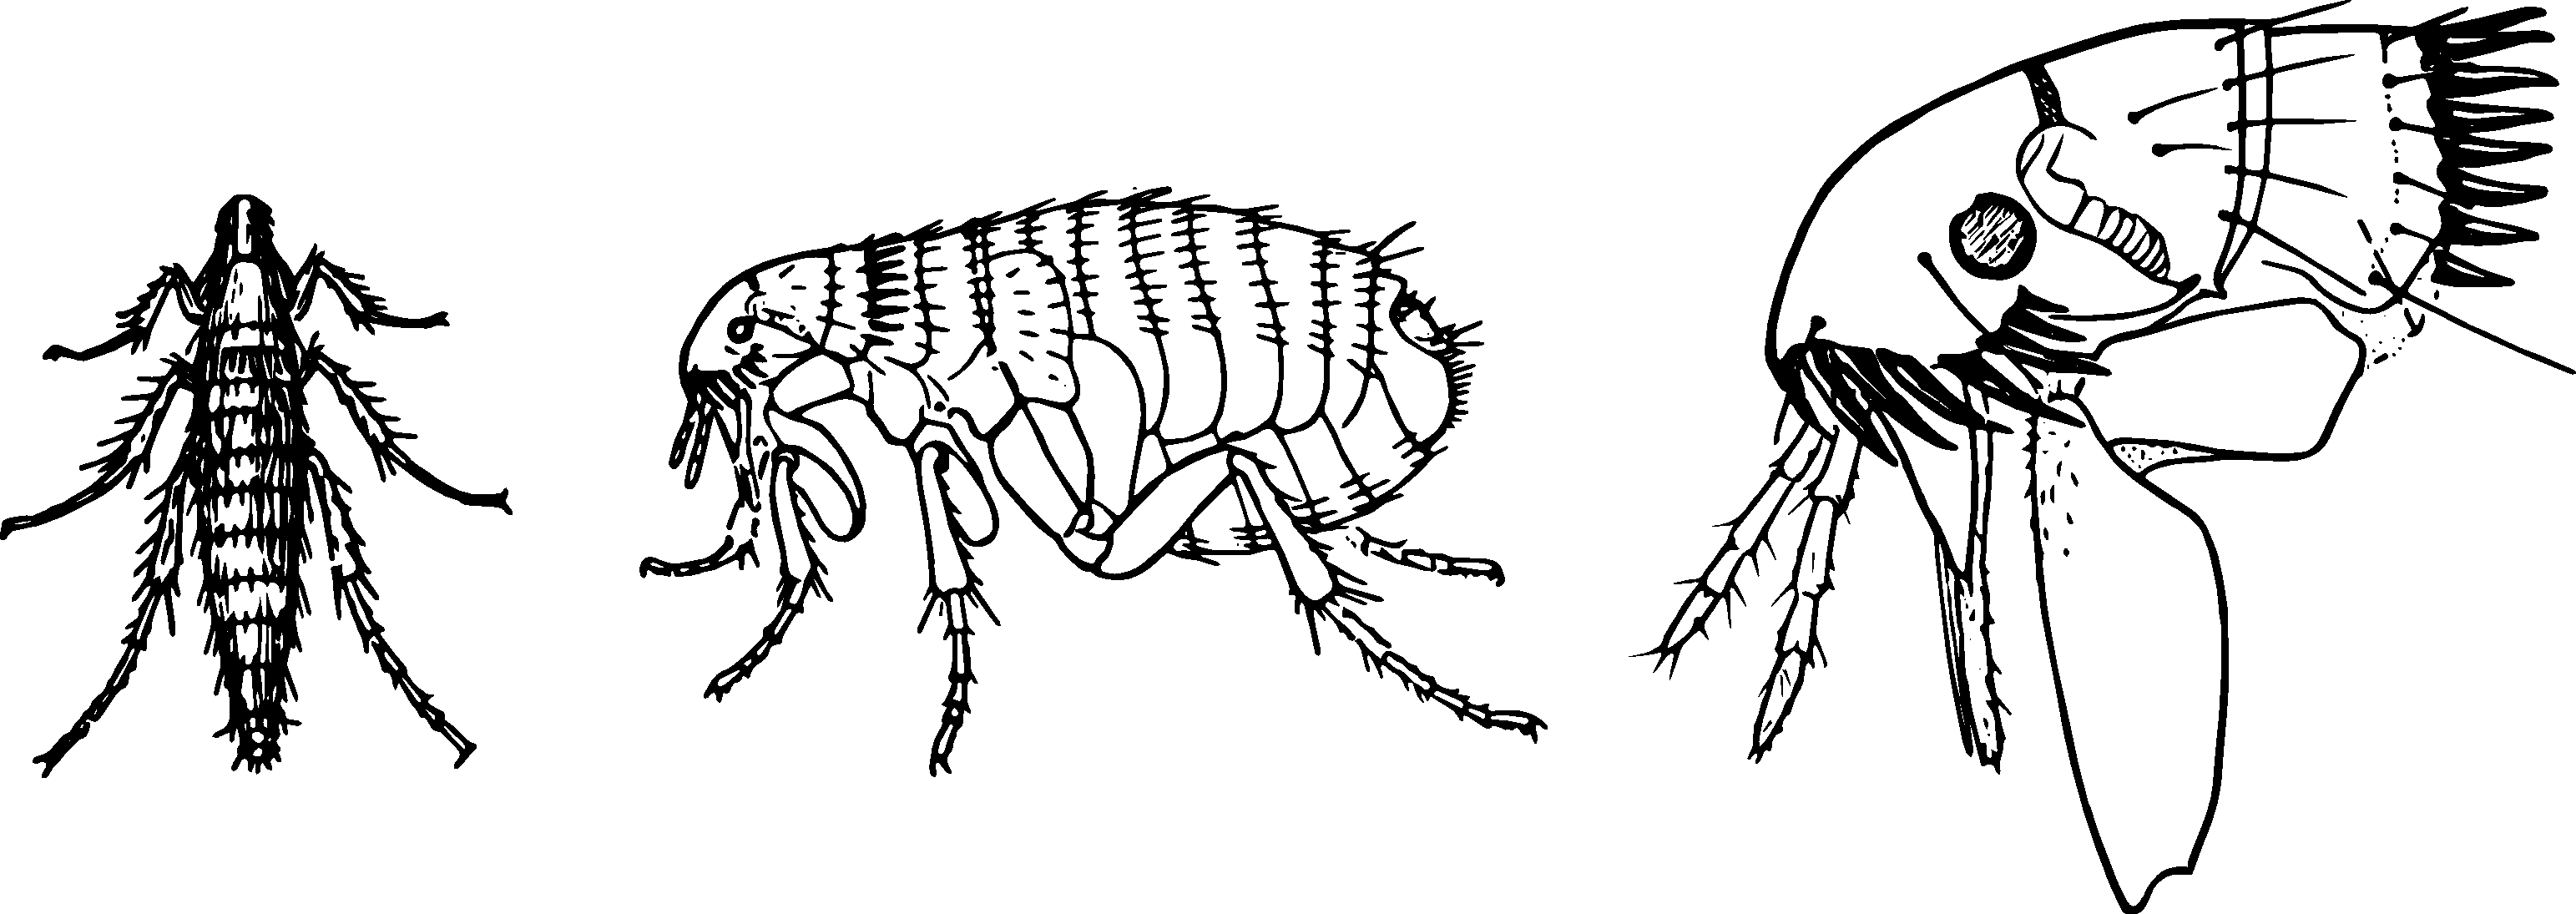
\includegraphics[width=0.75\textwidth]{antliophora/siphonaptera}}
  \caption{Siphonaptera \cite[modified from Figs. 33C--E in][]{snodgrass1944feeding}}
  \label{fig:pulicid}
\end{figure}

\section{Diptera (flies)}\index{Diptera}
\begin{itemize}
\item palps with 1--5 segments
\item 1--5 branches of R (Figure \ref{fig:dipteranwing})
\item hind wing (haltere) relatively small, knob-like
\end{itemize}

\begin{figure}[ht!]
  \centering
    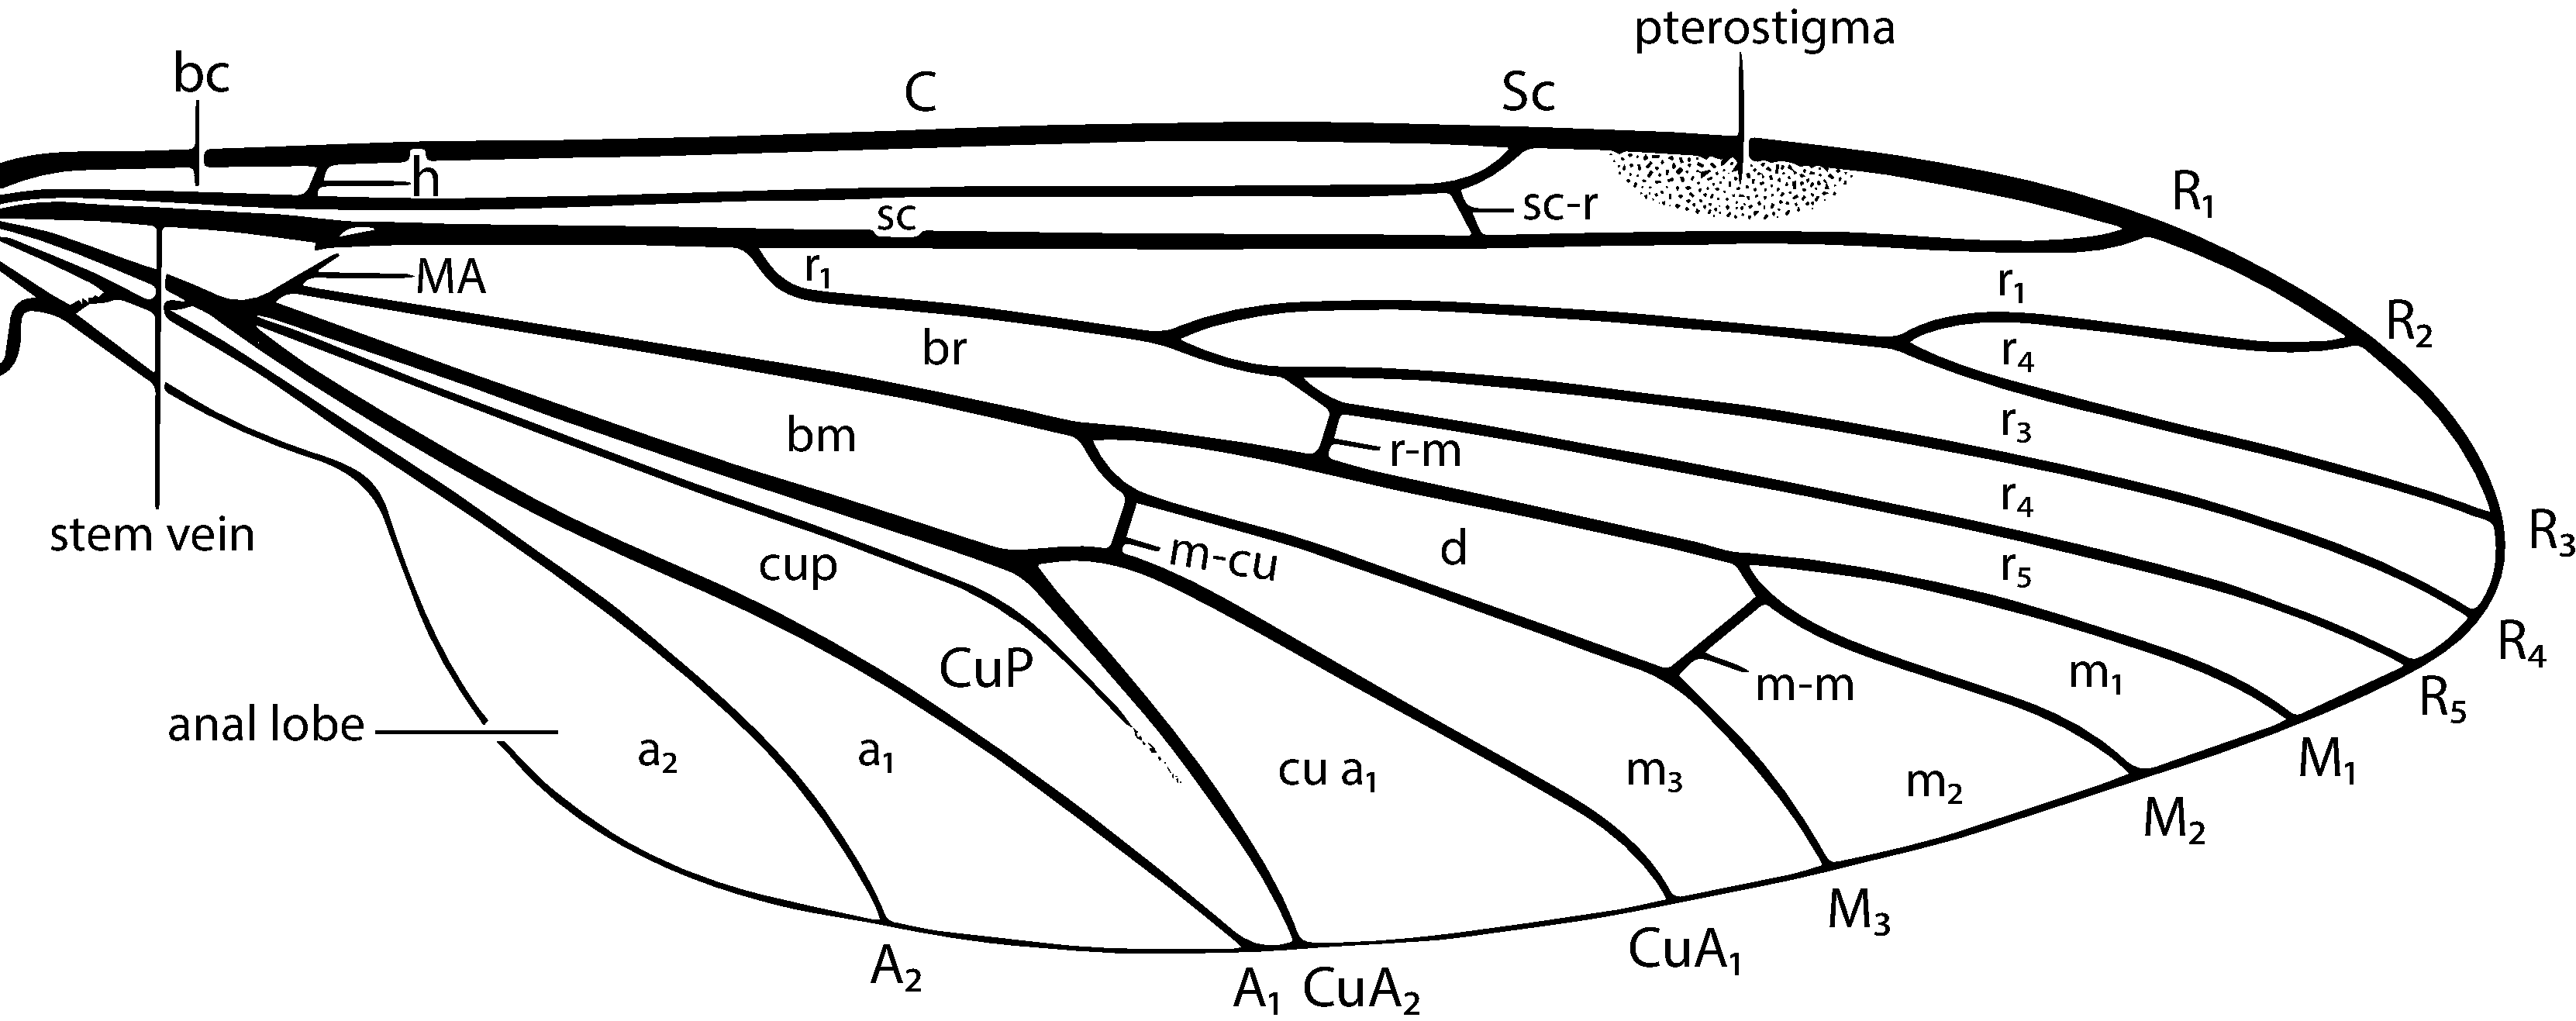
\includegraphics[width=0.75\textwidth]{antliophora/DipteraWing}
  \caption{Diptera, generalized fore wing \citep[][Fig. 67]{mcalpine1981manual}}
  \label{fig:dipteranwing}
\end{figure}

\subsection{Non-Brachycera (``Nematocera'')}\index{Nematocera}
\begin{itemize}
\item fragile, often with long legs 
\item antenna with 4+ freely articulated flagellomeres
\end{itemize}
This paraphyletic (hence the quotes around the name) group of taxa is comprised of species that have retained a lot of ancestral characters. 

\subsubsection{Tipulidae (crane flies)}\index{Tipulidae}
\noindent{}\textit{Diagnostic characters:} Ocelli absent; antennae slender but relatively short; mesonotum with V-shaped suture; wing with many veins; 2 anal veins reach margin; legs relatively long, autotomic (easily shed)\vspace{3mm}

\noindent{}\textit{Natural history:} Tipulids exhibit diverse life history strategies. many are aquatic, or nearly so, while others can be found as larvae in rotting wood and in decaying organic matter. Larvae are known to have diverse food habits; adults typically do not feed. More than 15,000 species have been described, most of them by the prolific taxonomist, C. P. Alexander.\vspace{3mm}

\begin{figure}[ht!]
    \centering
    \begin{subfigure}[ht!]{0.4\textwidth}
        \includegraphics[width=\textwidth]{antliophora/TipulidHabitus}
        \caption{}
        \label{fig:tipulid1}
    \end{subfigure}
    \qquad 
    \begin{subfigure}[ht!]{0.45\textwidth}
        \includegraphics[width=\textwidth]{antliophora/TipulidThorax}
        \caption{}
        \label{fig:tipulid2}
    \end{subfigure}
    \caption{Tipulidae. \textbf{(a)} Habitus \citep[][Fig. 7.1]{mcalpine1981manual}; \textbf{(b)} lateral thorax and head \citep[][Fig. 7.2]{mcalpine1981manual}}\label{fig:tipulids}
\end{figure}

\subsubsection{Simuliidae (black flies)}\index{Simuliidae}
\noindent{}\textit{Diagnostic characters:} Stout-bodied, humpbacked, \textless3 mm; ocelli absent; antennae as long as or shorter than head (but still filiform); wings broad, anterior veins thick, posterior veins weakly sclerotized.\vspace{3mm}

\noindent{}\textit{Natural history:} Black flies develop in lotic habitats, where they anchor themselves to rocks and feed on passing debris (algae, \textit{etc}.) The larvae are quite sensitive to disturbance. Adults are typically blood feeders. More than 1,800 species have been described worldwide.

\begin{figure}[ht!]
    \centering
    \begin{subfigure}[ht!]{0.32\textwidth}
        \includegraphics[width=\textwidth]{antliophora/SimuliidHead}
        \caption{}
        \label{fig:simuliid1}
    \end{subfigure}
    \qquad 
    \begin{subfigure}[ht!]{0.42\textwidth}
        \includegraphics[width=\textwidth]{antliophora/SimuliidHabitus}
        \caption{}
        \label{fig:simuliid2}
    \end{subfigure}
    \caption{Simuliidae. \textbf{(a)} Head \citep[][Fig. 27.5]{mcalpine1981manual}; \textbf{(b)} lateral thorax and head \citep[][Fig. 27.1]{mcalpine1981manual}}\label{fig:simuliids}
\end{figure}

\subsubsection{Chironomidae (midges)}\index{Chironomidae}%https://flic.kr/p/afohUk
\noindent{}\textit{Diagnostic characters:} Ocelli absent; antennae usually plumose, more so in males; mouthparts without mandibles; legs long, fore leg longer than others; fore wing M unbranched.\vspace{3mm}

\noindent{}\textit{Natural history:} Larval midges are generally aquatic, and species span the spectrum from highly sensitive to extremely tolerant of environmental disturbances. These flies feed on a variety of foods but generally not blood feeders. They also serve as important source of food for vertebrates. More than 10,000 species have been described worldwide.

\begin{figure}[ht!]
    \centering
    \begin{subfigure}[ht!]{0.45\textwidth}
        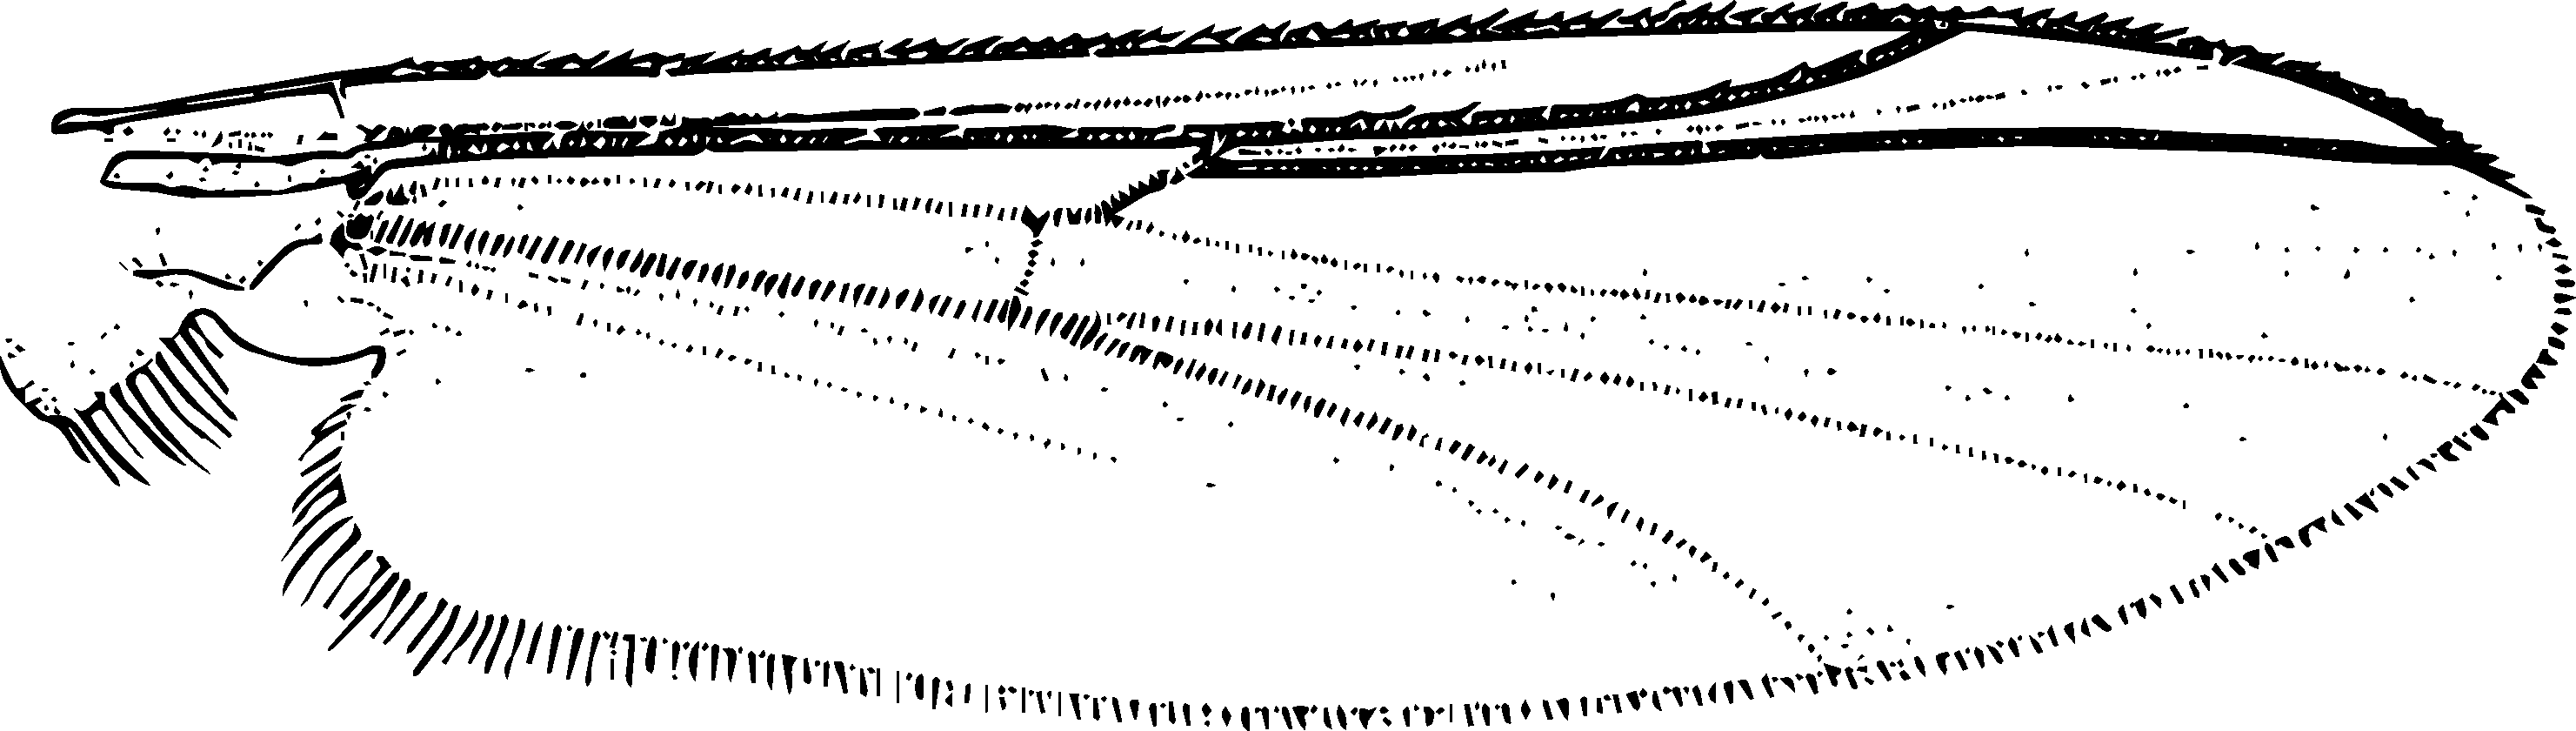
\includegraphics[width=\textwidth]{antliophora/ChironomidWing}
        \caption{}
        \label{fig:chiron1}
    \end{subfigure}
    \qquad 
    \begin{subfigure}[ht!]{0.45\textwidth}
        \includegraphics[width=\textwidth]{antliophora/ChironomidHabitus}
        \caption{}
        \label{fig:chiron2}
    \end{subfigure}
    \caption{Chironomidae. \textbf{(a)} Fore wing \citep[][Fig. 29.9]{mcalpine1981manual}; \textbf{(b)} habitus \citep[][Fig. 29.1]{mcalpine1981manual}}\label{fig:chironomids}
\end{figure}

\subsubsection{Ceratopogonidae (biting midges, no-see-ums, punkies)}\index{Ceratopogonidae}
\noindent{}\textit{Diagnostic characters:} Mouthparts with mandibles; ocelli mabsent; fore wing M branched into 2--3 veins; legs relatively short; similar to other nematocerans in habitus but usually much smaller (1--3 mm). \vspace{3mm}

\noindent{}\textit{Natural history:} These flies are generally found associated with aquatic or semi-aquatic habitats. Adults often feed on hemolymph, either from other insects or vertebrates. Some species are important vectors of disease. Adults are generally small (1--4 mm). More than 6,000 species have been described worldwide.  

\begin{figure}[ht!]
    \centering
    \begin{subfigure}[ht!]{0.35\textwidth}
        \includegraphics[width=\textwidth]{antliophora/CeratopogonidHead}
        \caption{}
        \label{fig:ceratopogonid1}
    \end{subfigure}
    \qquad 
    \begin{subfigure}[ht!]{0.5\textwidth}
        \includegraphics[width=\textwidth]{antliophora/CeratopogonidHabitus}
        \caption{}
        \label{fig:ceratopogonid2}
    \end{subfigure}
    \caption{Ceratopogonidae. \textbf{(a)} Head in anterior view \citep[][Fig. 28.4]{mcalpine1981manual}; \textbf{(b)} habitus \citep[][Fig. 28.13]{mcalpine1981manual}}\label{fig:ceratopogonids}
\end{figure}

\subsubsection{Culicidae (mosquitoes)}\index{Culicidae}
\noindent{}\textit{Diagnostic characters:} Body, especially wings often scaly; ocelli absent; proboscis long; antennae plumose, more so in males; wings narrow, with scales on veins.\vspace{3mm}

\noindent{}\textit{Natural history:} Mosquito larvae develop in aquatic habitats. Adult females feed on hemolymph, and many species are important vectors of disease, including malaria, Dengue, Zika, and West Nile virus. More than 3,700 species have been described worldwide.

\begin{figure}[ht!]
    \centering
    \begin{subfigure}[ht!]{0.45\textwidth}
        \includegraphics[width=\textwidth]{antliophora/CulicidWing}
        \caption{}
        \label{fig:culic1}
    \end{subfigure}
    \qquad
    \begin{subfigure}[ht!]{0.45\textwidth}
        \includegraphics[width=\textwidth]{antliophora/CulicidHabitus}
        \caption{}
        \label{fig:culic2}
    \end{subfigure}
    \caption{Culicidae. \textbf{(a)} Fore wing, with scales \citep[][Fig. 25.5]{mcalpine1981manual}; \textbf{(b)} habitus \citep[][Fig. 25.1]{mcalpine1981manual}}\label{fig:culicids}
\end{figure}

\subsubsection{Psychodidae (moth, sand, drain flies)}\index{Psychodidae}
\noindent{}\textit{Diagnostic characters:} Small to minute, stout and very setose;  antennae with characteristic setae rings; ocelli absent; wings broad oval, tapering apically, hairy, venation distinct; fore wing R 4-branched, with straight veins, few crossveins, and transverse fold near base of wing.\vspace{3mm}

\noindent{}\textit{Natural history:} Moth and sand fly larvae develop in habitats rich in organic matter and water, \textit{e.g.}, in drains. Phlebotominae are blood-feeders and can vector important diseases. More than 3,000 species have been described worldwide.

\begin{figure}[ht!]
    \centering
    \begin{subfigure}[ht!]{0.4\textwidth}
        \includegraphics[width=\textwidth]{antliophora/PsychodidWing}
        \caption{}
        \label{fig:psychodid1}
    \end{subfigure}
    \qquad
    \begin{subfigure}[ht!]{0.45\textwidth}
        \includegraphics[width=\textwidth]{antliophora/PsychodidHabitus}
        \caption{}
        \label{fig:psychodid2}
    \end{subfigure}
    \caption{Psychodidae. \textbf{(a)} Fore wing, with scales \citep[][Fig. 17.11]{mcalpine1981manual}; \textbf{(b)} habitus \citep[][Fig. 17.1]{mcalpine1981manual}}\label{fig:psychodids}
\end{figure}

\subsubsection{Cecidomyiidae (gall midges)}\index{Cecidomyiidae}
\noindent{}\textit{Diagnostic characters:} Eyes usually meet above antennae; wing venation reduced, \textless7 prominent veins reach margin; C continues around wing apex, though weaker posteriorly; first tarsal segment very small; antennae and legs long, slender; usually small (1--5 mm).\vspace{3mm}

\noindent{}\textit{Natural history:} As their common name suggests, these flies usually develop inside galls, where they feed on plant material. Some species, however, are important, free-roaming predators of other invertebrates. About 6,300 species have been described worldwide.

\begin{figure}[ht!]
    \centering
    \begin{subfigure}[ht!]{0.45\textwidth}
        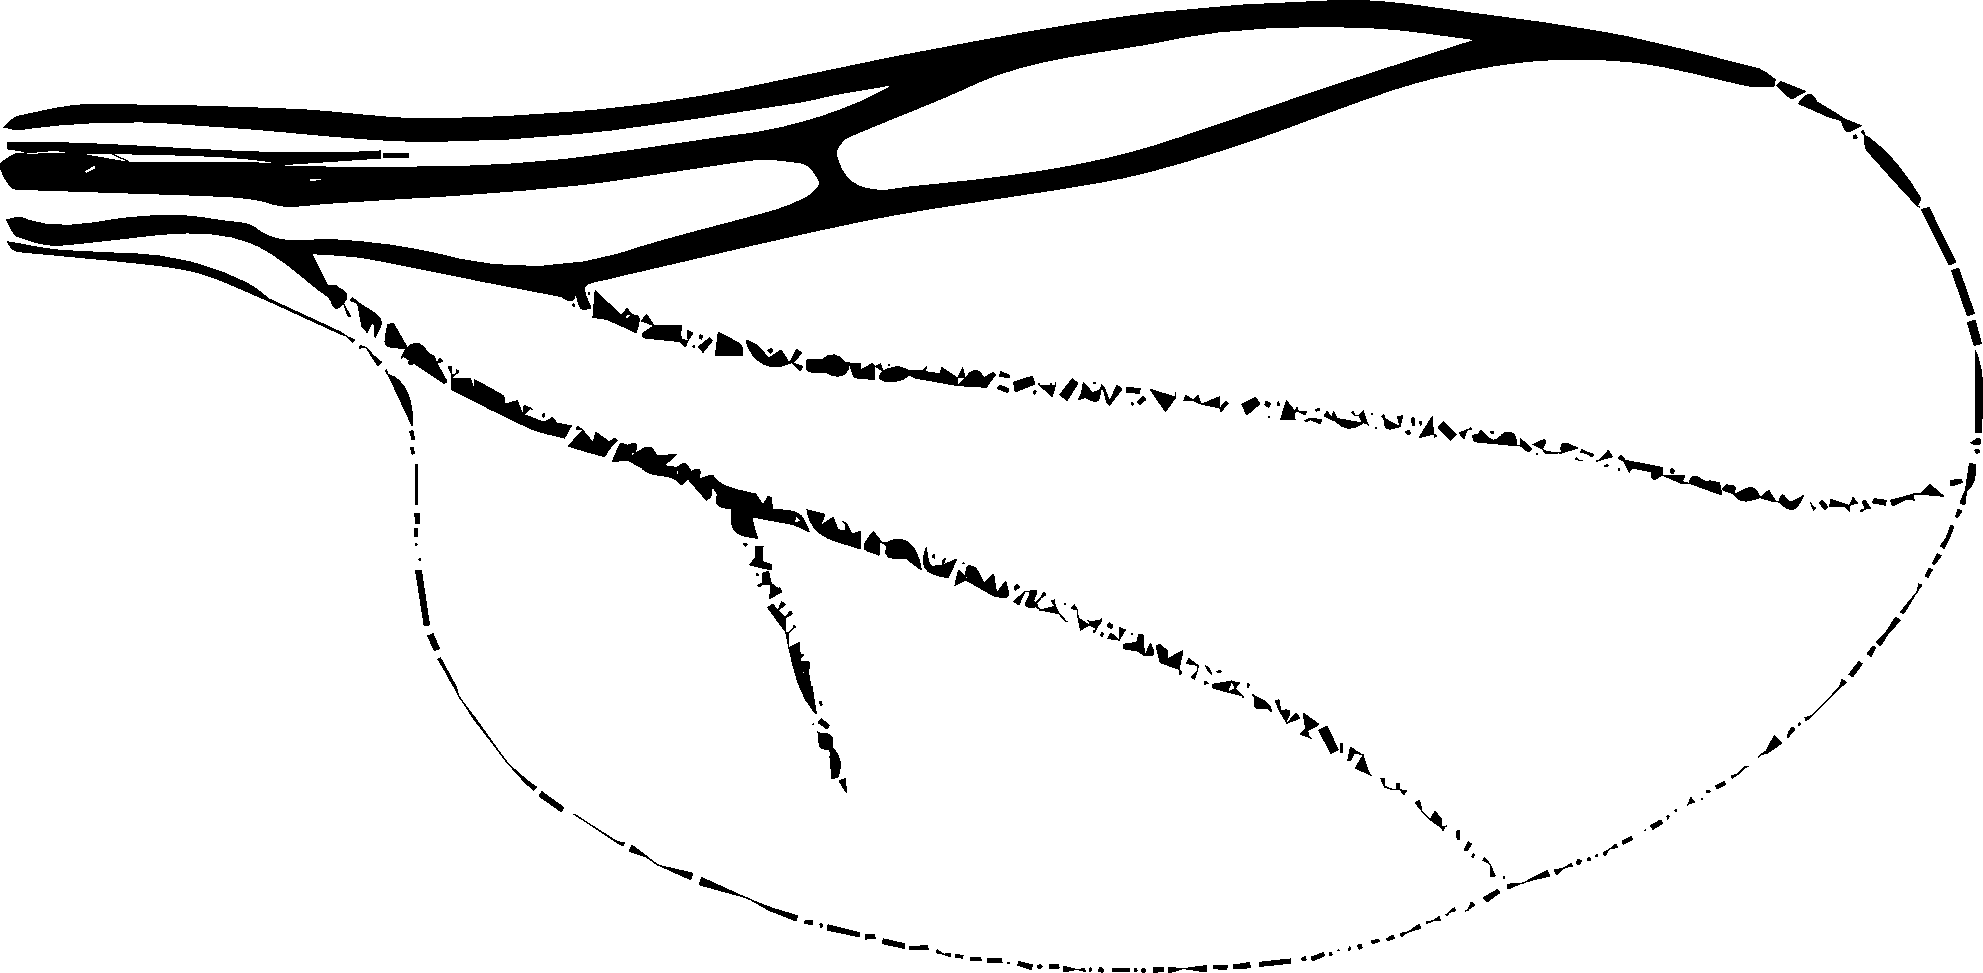
\includegraphics[width=\textwidth]{antliophora/CecidomyiidWing}
        \caption{}
        \label{fig:cecidomyiid1}
    \end{subfigure}
    \qquad
    \begin{subfigure}[ht!]{0.25\textwidth}
        \includegraphics[width=\textwidth]{antliophora/CecidomyiidHead}
        \caption{}
        \label{fig:cecidomyiid2}
    \end{subfigure}
    \caption{Cecidomyiidae. \textbf{(a)} Fore wing \citep[][Fig. 16.13]{mcalpine1981manual}; \textbf{(b)} habitus \citep[][Fig. 16.2]{mcalpine1981manual}}\label{fig:cecidomyiids}
\end{figure}

\subsubsection{Sciaridae (dark-winged fungus gnats)}\index{Sciaridae}
\noindent{}\textit{Diagnostic characters:} Usually mostly black or dark brown in color; eyes meet above antennae; ocelli present; wing venation reduced, usually \textless7 prominent veins reach margin; C ends at wing tip.\vspace{3mm}

\noindent{}\textit{Natural history:} Larvae generally feed on fungi, and some species are important pests of commercial mushrooms. More than 2,500 species have been described worldwide.

\begin{figure}[ht!]
    \centering
    \begin{subfigure}[ht!]{0.45\textwidth}
        \includegraphics[width=\textwidth]{antliophora/SciaridWing}
        \caption{}
        \label{fig:sciarid1}
    \end{subfigure}
    \qquad
    \begin{subfigure}[ht!]{0.25\textwidth}
        \includegraphics[width=\textwidth]{antliophora/SciaridHead}
        \caption{}
        \label{fig:sciarid2}
    \end{subfigure}
    \caption{Sciaridae. \textbf{(a)} Fore wing \citep[][Fig. 15.19]{mcalpine1981manual}; \textbf{(b)} habitus \citep[][Fig. 15.4]{mcalpine1981manual}}\label{fig:sciarids}
\end{figure}

\subsubsection{Mycetophilidae (fungus gnats)}\index{Mycetophilidae}
\noindent{}\textit{Diagnostic characters:} Head often concealed in dorsal view; ocelli present; antennae longer than thorax; eyes do not meet above antennae; coxae relatively elongate.\vspace{3mm}

\noindent{}\textit{Natural history:} With \textgreater4,500 species worldwide, these flies comprise another important group of fungivores. As with Sciaridae, adults are harmless.

\begin{figure}[ht!]
    \centering
    \begin{subfigure}[ht!]{0.45\textwidth}
        \includegraphics[width=\textwidth]{antliophora/MycetophilidWing}
        \caption{}
        \label{fig:mycetophilid1}
    \end{subfigure}
    \qquad
    \begin{subfigure}[ht!]{0.27\textwidth}
        \includegraphics[width=\textwidth]{antliophora/MycetophilidHead}
        \caption{}
        \label{fig:mycetophilid2}
    \end{subfigure}
    \caption{Mycetophilidae. \textbf{(a)} Fore wing \citep[][Fig. 14.24]{mcalpine1981manual}; \textbf{(b)} head in lateral view \citep[][Fig. 13.1]{mcalpine1981manual}}\label{fig:mycetophilids}
\end{figure}

\subsubsection{Bibionidae (March flies)}\index{Bibionidae}
\noindent{}\textit{Diagnostic characters:} Body with many erect bristles (\textit{i.e.}, ``hairy''), usually black; male head shape different from female; ocelli present; antennae shorter than thorax, arising low on face; basal M cell present; anal angle of wing somewhat enlarged.\vspace{3mm}

\noindent{}\textit{Natural history:} Larvae feed in leaf litter and topsoil on decaying organic matter. Adults emerge in spring or fall and often form large mating swarms. In some regions (\textit{e.g.}, Florida) these flies are referred to as ``love bugs''. About 1,200 species have been described worldwide.

\begin{figure}[ht!]
    \centering
    \begin{subfigure}[ht!]{0.25\textwidth}
        \includegraphics[width=\textwidth]{antliophora/BibionidHead}
        \caption{}
        \label{fig:bibionid1}
    \end{subfigure}
    \qquad
    \begin{subfigure}[ht!]{0.47\textwidth}
        \includegraphics[width=\textwidth]{antliophora/BibionidHabitus}
        \caption{}
        \label{fig:bibionid2}
    \end{subfigure}
    \caption{Bibionidae. \textbf{(a)} Female head in lateral view \citep[][Fig. 13.3]{mcalpine1981manual}; \textbf{(b)} male habitus \citep[][Fig. 13.1]{mcalpine1981manual}}\label{fig:bibionids}
\end{figure}

\subsection{Brachycera (short-horned flies)}\index{Brachycera}
\begin{itemize}
\item generally stouter bodied than ``Nematocera''
\item flagellum at least partly fused, with \textless5 articulations, very rarely \textgreater10
\item palps with 0--2 segments
\end{itemize}
Unlike ``Nematocera'', this suborder is demonstrably monophyletic. There have been several attempts to subdivide this taxon, but each scheme usually results in one paraphyletic group and one monophyletic group.

\subsubsection{Stratiomyidae (soldier flies)}\index{Stratiomyidae}
\noindent{}\textit{Diagnostic characters:} Often mimics of wasps or bees; 3rd antennal segment elongate, annulate or rounded, with arista; fore wing d cell round, not elongate, Rs bunched near anterior margin, R4 and R5 fork anterior to wing tip, C ends before wing tip.\vspace{3mm}

\noindent{}\textit{Natural history:} Larvae generally feed on decaying plants, and maggots can frequently be found in compost bins. Some species are aquatic. About 2,700 species have been described worldwide.

\begin{figure}[ht!]
    \centering
    \begin{subfigure}[ht!]{0.5\textwidth}
        \includegraphics[width=\textwidth]{antliophora/StratiomyidWing}
        \caption{}
        \label{fig:stratiomyid1}
    \end{subfigure}
    \qquad
    \begin{subfigure}[ht!]{0.2\textwidth}
        \includegraphics[width=\textwidth]{antliophora/StratiomyidAntennae}
        \caption{}
        \label{fig:stratiomyid2}
    \end{subfigure}
    \caption{Stratiomyidae. \textbf{(a)} Fore wing \citep[][Fig. 36.33]{mcalpine1981manual}; \textbf{(b)} antenna variation \citep[][Figs. 36.9,12,15,18]{mcalpine1981manual}}\label{fig:stratiomyids}
\end{figure}

\subsubsection{Tabanidae (horse and deer flies)}\index{Tabanidae}
\noindent{}\textit{Diagnostic characters:} Mouthparts modified for sucking blood and nectar; eyes often with iridescent patterns; 3rd antennal segment never aristate; fore wing R4 and R5 fork encloses wing tip, d cell elongate; postscutellum present; first visible abdominal tergite divided dorsally.\vspace{3mm}

\noindent{}\textit{Natural history:} Larvae are predators and can usually be found in/near aquatic habitats. Adult females are usually blood feeders, and some can vector important human diseases (\textit{e.g.}, \textit{Loa loa}).Approximately 4,500 species have been described worldwide.

\begin{figure}[ht!]
    \centering
    \begin{subfigure}[ht!]{0.4\textwidth}
        \includegraphics[width=\textwidth]{antliophora/TabanidWing}
        \caption{}
        \label{fig:tabanid1}
    \end{subfigure}
    \qquad
    \begin{subfigure}[ht!]{0.5\textwidth}
        \includegraphics[width=\textwidth]{antliophora/TabanidHabitus}
        \caption{}
        \label{fig:tabanid2}
    \end{subfigure}
    \caption{Tabanidae. \textbf{(a)} Fore wing \citep[][Fig. 31.35]{mcalpine1981manual}; \textbf{(b)} habitus \citep[][Fig. 31.1]{mcalpine1981manual}}\label{fig:tabanids}
\end{figure}

\subsubsection{Asilidae (robber flies)}\index{Asilidae}
\noindent{}\textit{Diagnostic characters:} Medium-sized to large flies, variable but often mimicking bees or with elongate, tapering abdomen; top of head (vertex) distinctly depressed between eyes; face with mystax (mustache); mouthparts heavily sclerotized, pointed, for piercing; fore wing CuA2 reaches wing margin or joins A1 near margin.\vspace{3mm}

\noindent{}\textit{Natural history:} Larval asilids usually develop in rotting wood or leaf litter, where they develop as predators or saprophages. Adults are effective predators of other insects, often larger than themselves. More than 7,000 species have been described worldwide.

\begin{figure}[ht!]
    \centering
    \begin{subfigure}[ht!]{0.25\textwidth}
        \includegraphics[width=\textwidth]{antliophora/AsilidHead}
        \caption{}
        \label{fig:asilid2}
    \end{subfigure}
    \qquad 
    \begin{subfigure}[ht!]{0.45\textwidth}
        \includegraphics[width=\textwidth]{antliophora/AsilidHabitus}
        \caption{}
        \label{fig:asilid1}
    \end{subfigure}
    \caption{Asilidae. \textbf{(a)} Head \citep[][Fig. 42.35]{mcalpine1981manual}; \textbf{(b)} habitus \citep[][Fig. 42.1]{mcalpine1981manual}}\label{fig:asilids}
\end{figure}

\subsubsection{Bombyliidae (bee flies)}\index{Bombyliidae}
\noindent{}\textit{Diagnostic characters:} Extremely variable in form and size but commonly hairy and stout, mimicking bees; proboscis often slender and long;; wing venation variable but veins often strongly curved anteriorly; CuA2 reaches wing margin or joins A1 near margin; cell bm with 3 corners on the end.\vspace{3mm}

\noindent{}\textit{Natural history:} About 4,500 bee flies have been described worldwide, the majority of which are assumed to develop as cleptoparasites, predators, and/or parasitoids of insects that live in burrows (\textit{e.g.}, solitary bees).

\begin{figure}[ht!]
    \centering
    \begin{subfigure}[ht!]{0.45\textwidth}
        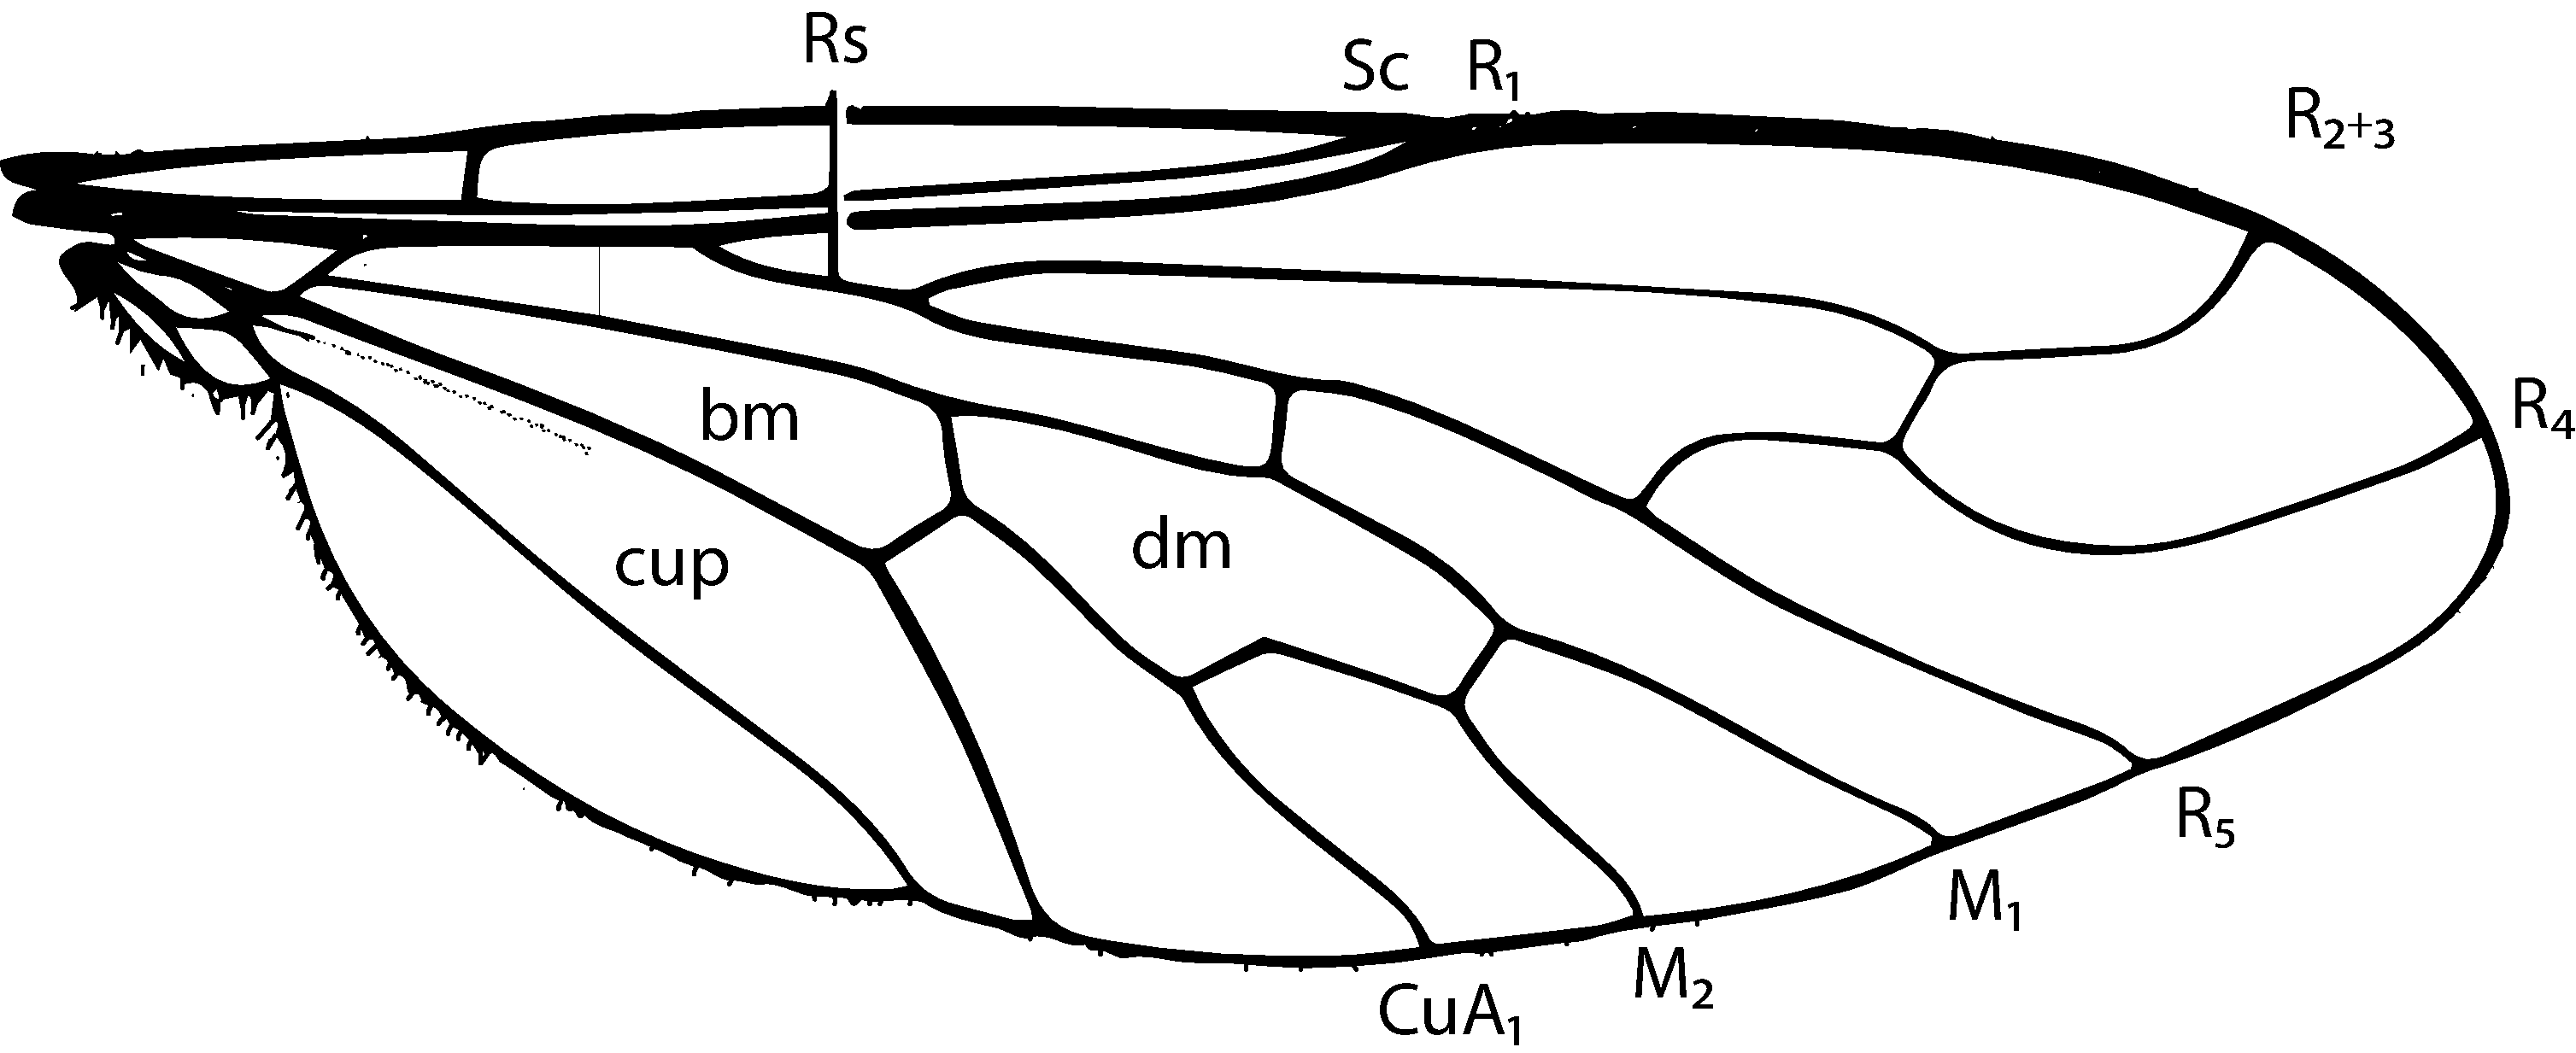
\includegraphics[width=\textwidth]{antliophora/BombyliidWing}
        \caption{}
        \label{fig:bombyl2}
    \end{subfigure}
    \qquad 
    \begin{subfigure}[ht!]{0.4\textwidth}
        \includegraphics[width=\textwidth]{antliophora/BombyliidHabitus}
        \caption{}
        \label{fig:bombyl1}
    \end{subfigure}
    \caption{Bombyliidae. \textbf{(a)} Fore wing \citep[][Fig. 45.1]{mcalpine1981manual}; \textbf{(b)} habitus \citep[][Fig. 45.1]{mcalpine1981manual}}\label{fig:bombyls}
\end{figure}

\paragraph{Eremoneura} The remaining flies belong to Eremoneura and are characterized, in part, by having three larval instars and relatively few wing veins.\index{Eremoneura}

\subsubsection{Dolichopodidae (long-legged flies)}\index{Dolichopodidae}
\noindent{}\textit{Diagnostic characters:} Long-legged and usually metallic green or coppery; head shape is distinctive; antennae usually aristate; CuA2 joins A1 far from margin; Rs 2-branched, branches, r-m crossvein crowded near wing base, anal cell small or absent; male genitalia often large and folded under abdomen.\vspace{3mm}

\noindent{}\textit{Natural history:} Adult dolichopodids and most larvae  develop as predators of other insects; some larvae, however, are phytophagous. Abut 7,000 species have been described worldwide.

\begin{figure}[ht!]
    \centering
    \begin{subfigure}[ht!]{0.5\textwidth}
        \includegraphics[width=\textwidth]{antliophora/DolichopodidWing}
        \caption{}
        \label{fig:dolicho1}
    \end{subfigure}
    \qquad
    \begin{subfigure}[ht!]{0.22\textwidth}
        \includegraphics[width=\textwidth]{antliophora/DolichopodidHead}
        \caption{}
        \label{fig:dolicho2}
    \end{subfigure}
    \caption{Dolichopodidae. \textbf{(a)} Fore wing \citep[][Fig. 48.30]{mcalpine1981manual}; \textbf{(b)} head \citep[][Fig. 48.4]{mcalpine1981manual}}\label{fig:dolichos}
\end{figure}

\subsubsection{Empididae (dance flies)}\index{Empididae}
\noindent{}\textit{Diagnostic characters:} Body variable in shape but usually hump-backed, dome-shaped, and colorful but not metallic; 3rd antennal stylate or aristate; mouthparts extended into prominent beak-like structure, oriented ventrally; CuA2 joins A1 far from margin (look for large open cell in lower part of wing); wing venation otherwise variable, R 2--3-branched, branches and r-m crossvein arise distally.\vspace{3mm}

\noindent{}\textit{Natural history:} Adults and larvae of this family are thought to be predators of other insects. larvae are generally found inleaf litter and rotting wood, while adults are most frequently collected in mating swarms. Males usually present females with prey as nuptial gifts, although in some species simply present silken balloons. More than 3,100 species have been described worldwide.

\begin{figure}[ht!]
    \centering
    \begin{subfigure}[ht!]{0.45\textwidth}
        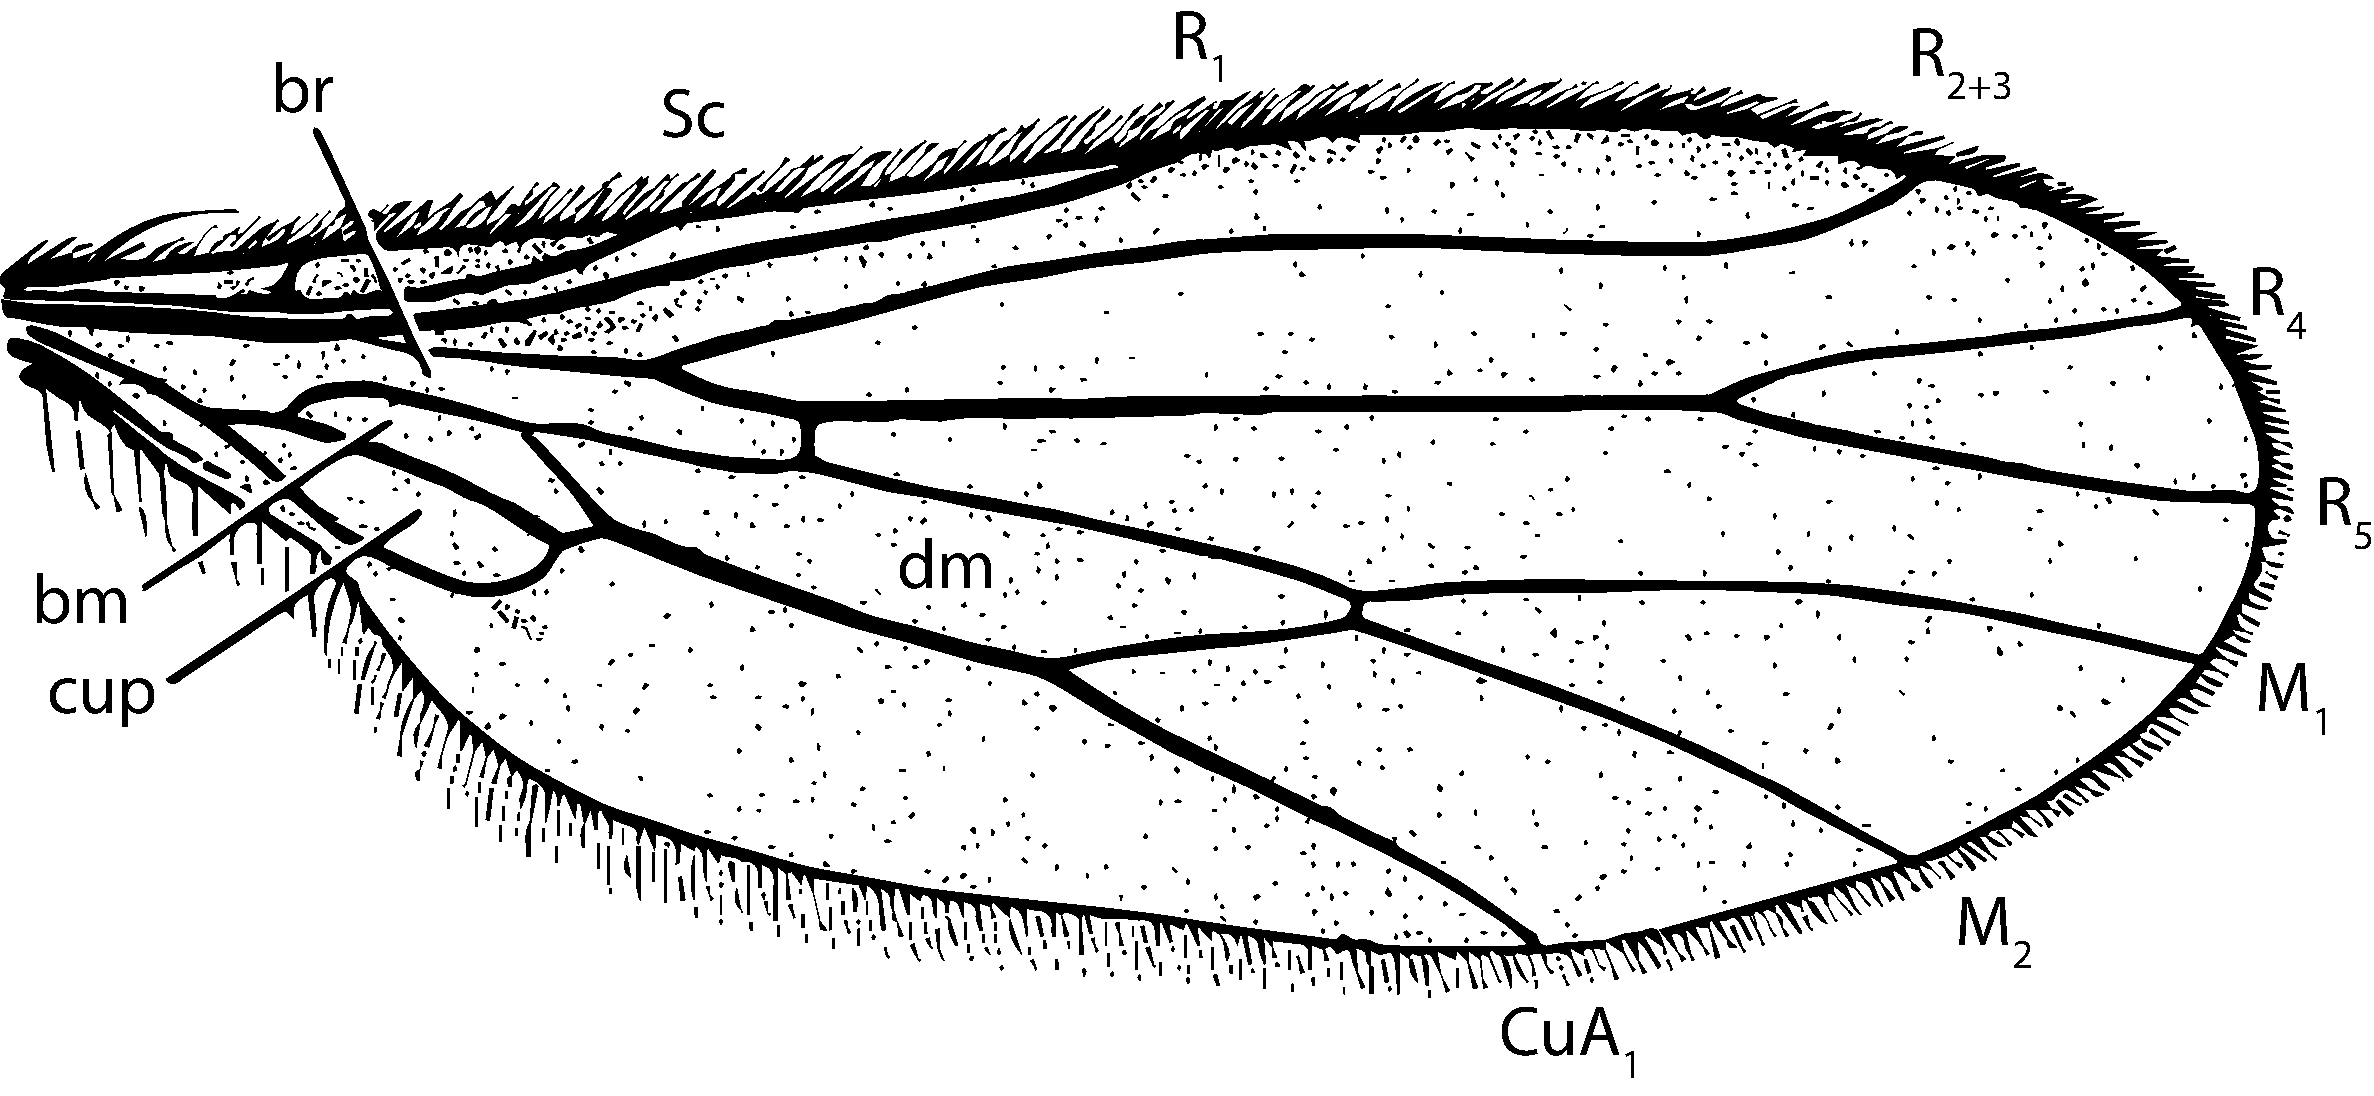
\includegraphics[width=\textwidth]{antliophora/EmpididWing}
        \caption{}
        \label{fig:empidid1}
    \end{subfigure}
    \qquad
    \begin{subfigure}[ht!]{0.42\textwidth}
        \includegraphics[width=\textwidth]{antliophora/EmpididHabitus}
        \caption{}
        \label{fig:empidid2}
    \end{subfigure}
    \caption{Empididae. \textbf{(a)} Fore wing \citep[][Fig. 47.24]{mcalpine1981manual}; \textbf{(b)} habitus \citep[][Fig. 47.1]{mcalpine1981manual}}\label{fig:empidids}
\end{figure}

\paragraph{Cyclorrhapha} The remaining flies are classified in Cyclorrhapha, which includes all flies that have circular opercula on their puparia (pupa inside exuviae), through which they escape during eclosion.\index{Cyclorrhapha}

\subsubsection{Syrphidae (hover, drone flies)}\index{Syrphidae}
\noindent{}\textit{Diagnostic characters:} CuA2 reaches wing margin or joins A1 near margin; spurious vein present in wing between R and M; M1 usually curves up to meet R4+5; antennae variable, often aristate; many mimic wasps and bees.\vspace{3mm}

\noindent{}\textit{Natural history:} About 6,000 species of hoverflies have been described worldwide, and larvae develop usually as predators (mainly of soft-bodied prey, like aphids) or saprophages. Adults are adept fliers that frequently mimic aculeate wasps.

\begin{figure}[ht!]
    \centering
    \begin{subfigure}[ht!]{0.45\textwidth}
        \includegraphics[width=\textwidth]{antliophora/SyrphidWing}
        \caption{}
        \label{fig:syrphid2}
    \end{subfigure}
    \qquad 
    \begin{subfigure}[ht!]{0.45\textwidth}
        \includegraphics[width=\textwidth]{antliophora/SyrphidHabitus}
        \caption{}
        \label{fig:syrpidh1}
    \end{subfigure}
    \caption{Syrphidae. \textbf{(a)} Fore wing \citep[][Fig. 52.52]{mcalpine1981manualv2}; \textbf{(b)} habitus \citep[][Fig. 52.1]{mcalpine1981manualv2}}\label{fig:syrphids}
\end{figure}

\subsubsection{Phoridae (scuttle, coffin flies, \textit{etc}.)}\index{Phoridae}
\noindent{}\textit{Diagnostic characters:} CuA2 joins A1 far from margin; wings very distinct; Rs crowded anteriorly, 4--5 weak veins posteriorly; antennae flagellum globular with long arista; hind femora flattened; body somewhat humpbacked.\vspace{3mm}

\noindent{}\textit{Natural history:} Scuttle flies are extraordinarily diverse ecologically, feeding on organic matter in just about every stage/state/derivation. Some feed on decaying plants, others on dying insects, others are parasitoids, \textit{etc}. About 4,000 species have been described, but tens of thousands remain to be described.

\begin{figure}[ht!]
    \centering
    \begin{subfigure}[ht!]{0.45\textwidth}
        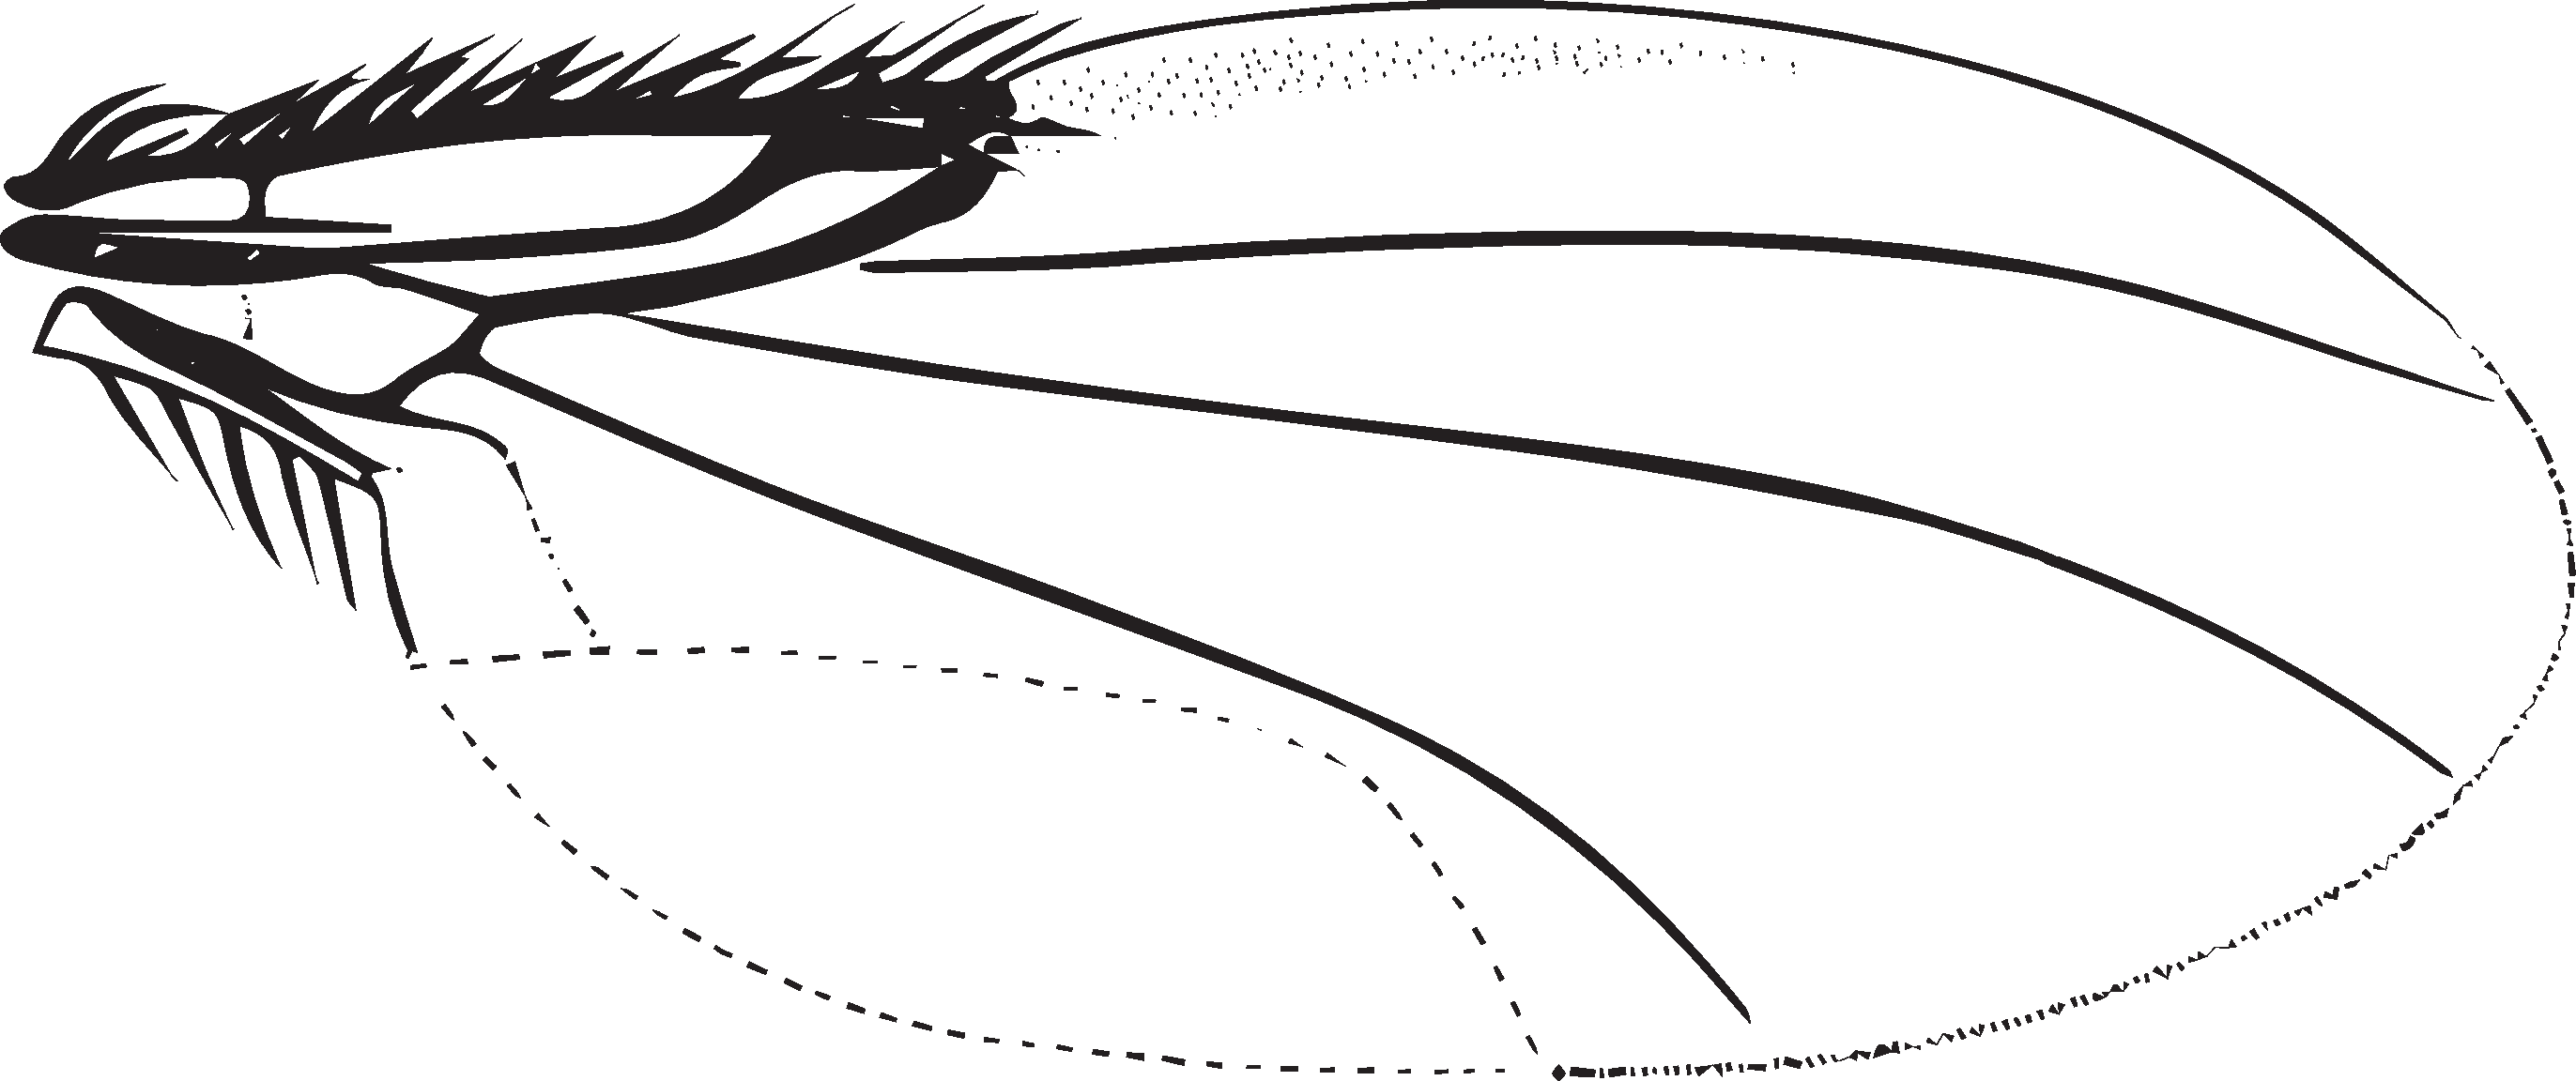
\includegraphics[width=\textwidth]{antliophora/PhoridWing}
        \caption{}
        \label{fig:phorid1}
    \end{subfigure}
    \qquad
    \begin{subfigure}[ht!]{0.45\textwidth}
        \includegraphics[width=\textwidth]{antliophora/PhoridHabitus}
        \caption{}
        \label{fig:phorid2}
    \end{subfigure}
    \caption{Phoridae. \textbf{(a)} Fore wing \citep[][Fig. 51.44]{mcalpine1981manualv2}; \textbf{(b)} habitus \citep[][Fig. 51.1]{mcalpine1981manualv2}}\label{fig:phorids}
\end{figure}

\paragraph{Schizophora} This taxon is thought to be monophyletic. It is comprised of species that usually share the following characteristics: \index{Schizophora}
\begin{itemize}
\item ptilinal suture (= frontal suture) present above the antennae; corresponds to structure (ptilinum) used to break out of puparium
\item CuA2 joins A1 far from margin
\item antennae almost always aristate
\end{itemize}
This taxon has traditionally been divided into two taxa, Acalyptratae and Calyptratae, based, in part, on the morphology of the fore wing. See below.

\paragraph{``Acalyptratae''} The next several families (before we enter Calyptratae) are commonly referred to as ``acalypterate flies'', a notoriously difficult group of flies to diagnose at almost any level. They generally share these character states:\index{Acalyptratae}
\begin{itemize}
\item calypter almost always small to absent (figure \ref{fig:acalypteratewing})
\item transverse suture on thorax almost always absent
\item greater ampulla usually absent (bump near wing base, anterior to calypters)
\item antennal pedicel usually without complete dorsal seam
\item generally smaller and less setose than calyptrates
\end{itemize}

\begin{figure}[ht!]
  \centering
    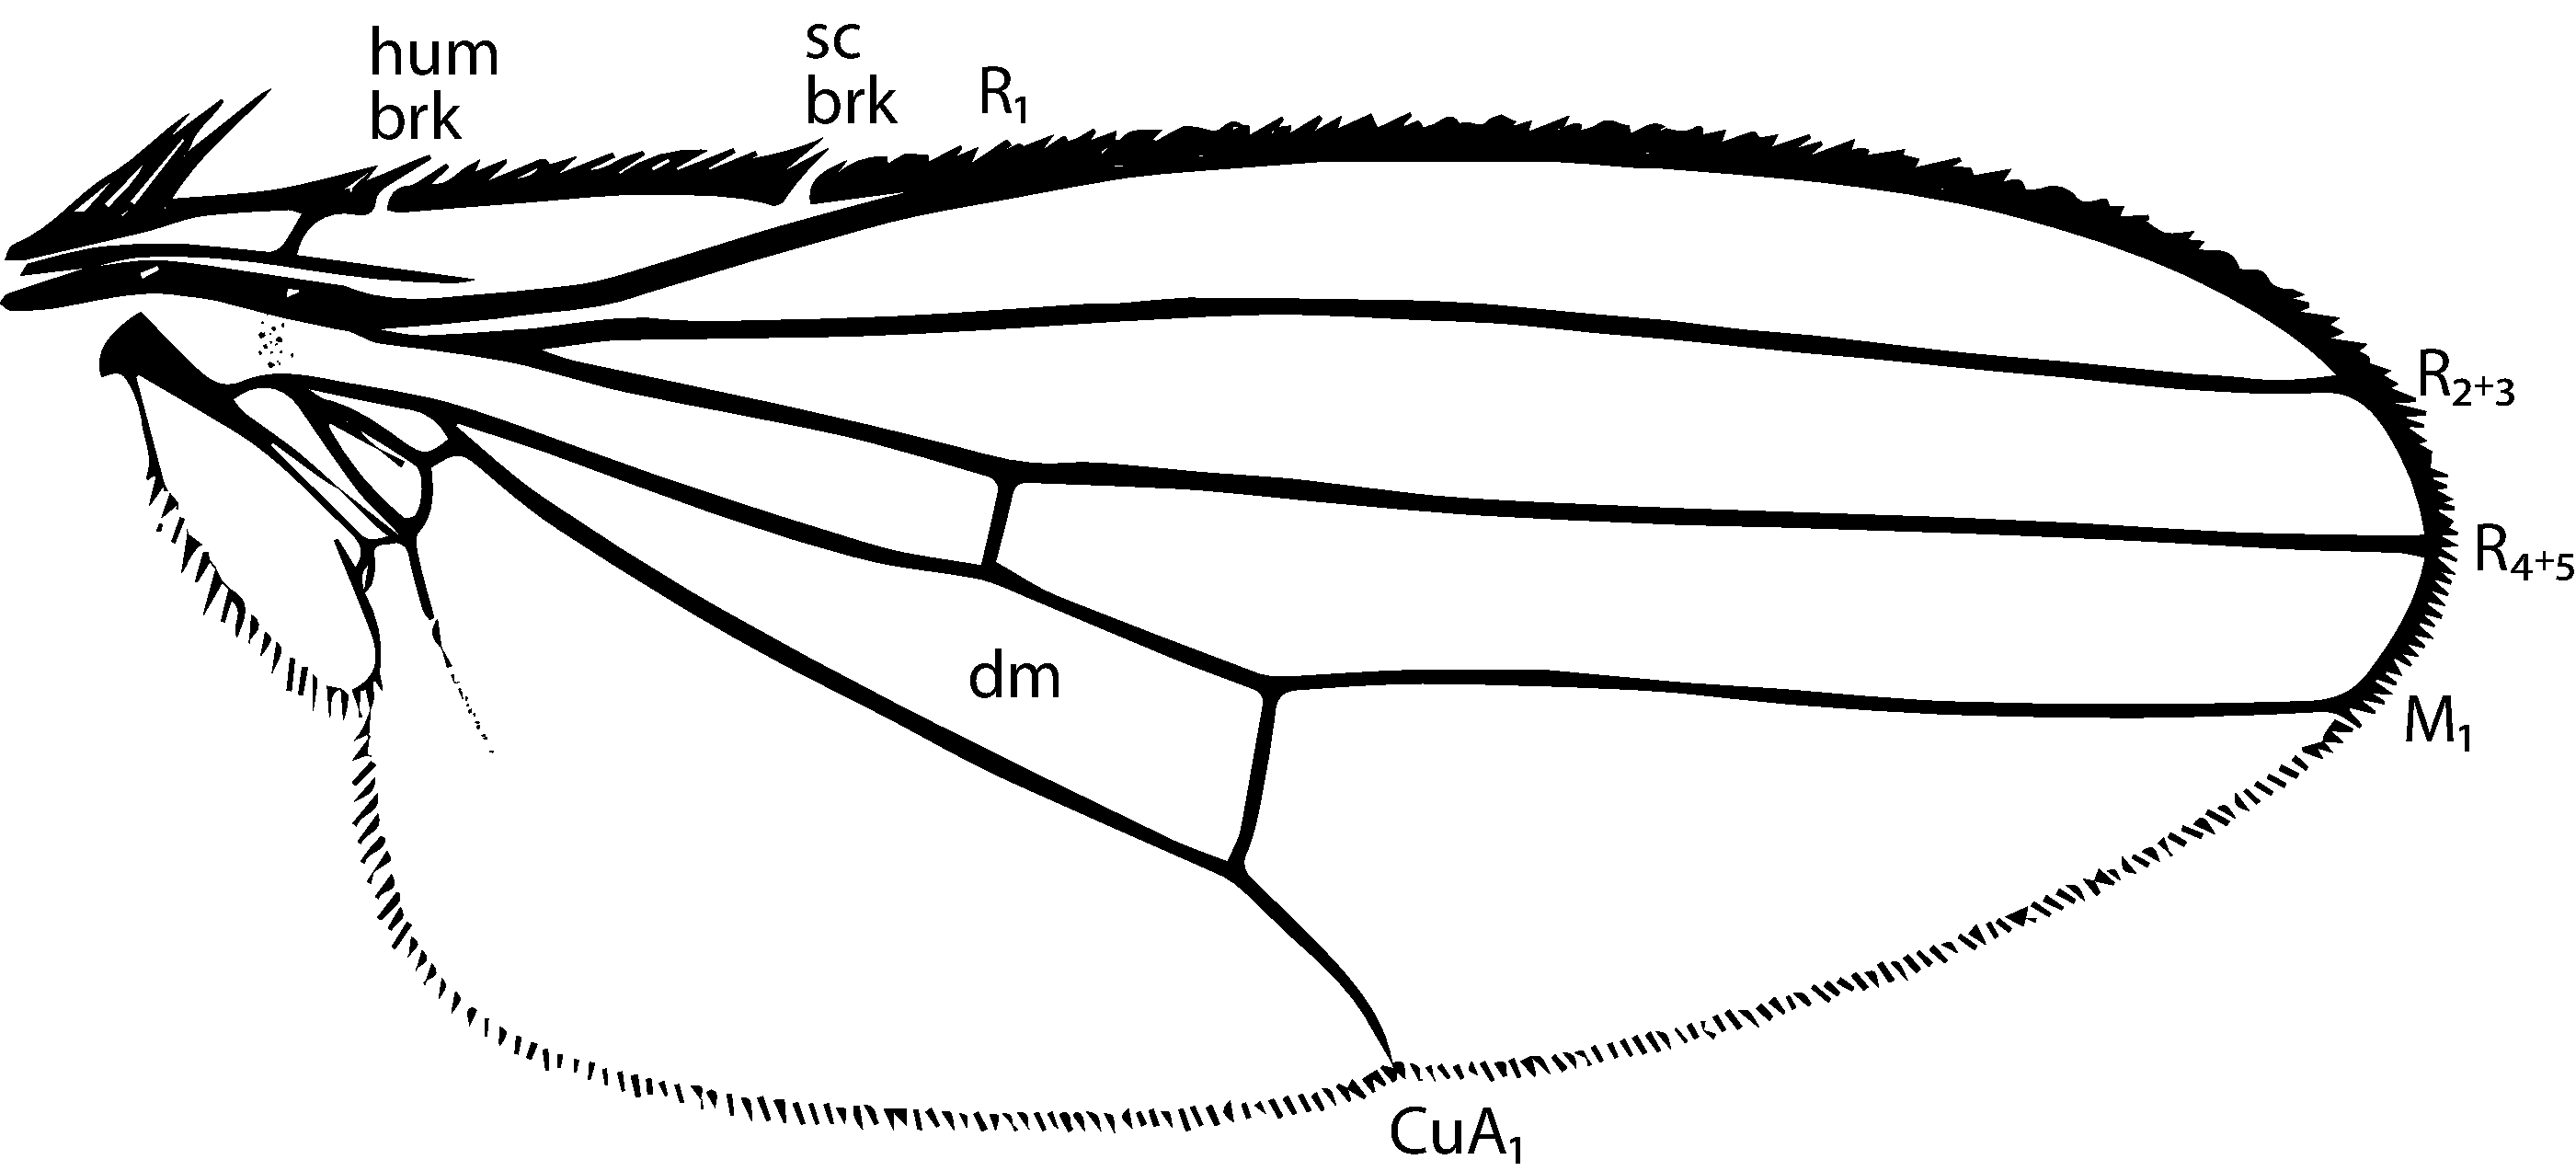
\includegraphics[width=0.5\textwidth]{antliophora/AcalyptrateWing}
  \caption{Reference acalypterate wing \citep[][Fig. 4.59]{mcalpine1981manual}}
  \label{fig:acalypteratewing}
\end{figure}

\subsubsection{Ulidiidae (picture-winged flies)}\index{Ulidiidae}
\noindent{}\textit{Diagnostic characters:} Sc complete, C usually entire; anal cell (cup in figure \ref{fig:ulidiid1}) usually with acute projection posteriorly; apex of Sc not bending abruptly; oral vibrissae lacking (figure \ref{fig:ulidiid2}); small to medium-sized, wings usually patterned.\vspace{3mm}

\noindent{}\textit{Natural history:} Larvae typically develop as saprophages or herbivores. Approximately 700 species have been described worldwide. Some resources still refer to this family as Otitidae.

\begin{figure}[ht!]
    \centering
    \begin{subfigure}[ht!]{0.47\textwidth}
        \includegraphics[width=\textwidth]{antliophora/UlidiidWing}
        \caption{}
        \label{fig:ulidiid1}
    \end{subfigure}
    \qquad
    \begin{subfigure}[ht!]{0.26\textwidth}
        \includegraphics[width=\textwidth]{antliophora/UlidiidHead}
        \caption{}
        \label{fig:ulidiid2}
    \end{subfigure}
    \caption{Ulidiidae. \textbf{(a)} Fore wing \citep[][Fig. 63.15]{mcalpine1981manualv2}; \textbf{(b)} head \citep[][Fig. 63.7]{mcalpine1981manualv2}}\label{fig:ulidiids}
\end{figure}

\subsubsection{Tephritidae (fruit flies)}\index{Tephritidae}
\noindent{}\textit{Diagnostic characters:} Sc usually incomplete, C usually broken; apex of Sc bent abruptly at end; small to medium-sized, often patterned on wings, sometimes also on body; anal cell sometimes with acute projection (as in Ulidiidae).\vspace{3mm}

\noindent{}\textit{Natural history:} The number of described species of fruit flies is approaching 5,000, which includes several significant pests. Larvae develop inside fruit, flowers, galls, and other plant parts. Note that this family does \textit{not} include \textit{Drosophila}, which are often referred to incorrectly as ``fruit flies''. 

\begin{figure}[ht!]
    \centering
    \begin{subfigure}[ht!]{0.45\textwidth}
        \includegraphics[width=\textwidth]{antliophora/TephritidWing}
        \caption{}
        \label{fig:tephritid1}
    \end{subfigure}
    \qquad
    \begin{subfigure}[ht!]{0.4\textwidth}
        \includegraphics[width=\textwidth]{antliophora/TephritidHabitus}
        \caption{}
        \label{fig:tephritid2}
    \end{subfigure}
    \caption{Tephritidae. \textbf{(a)} Fore wing \citep[][Fig. 4.56]{mcalpine1981manual}; \textbf{(b)} habitus \citep[][Fig. 66.1]{mcalpine1981manualv2}}\label{fig:tephritids}
\end{figure}

\subsubsection{Agromyzidae (leafminer flies)}\index{Agromyzidae}
\noindent{}\textit{Diagnostic characters:} Sc incomplete, costa broken once; anal cell present; oral vibrissae present; postvertical bristles diverging; small, usually black and/or yellow, bristly.\vspace{3mm}

\noindent{}\textit{Natural history:} Most agromyzids feed as larvae inside leaves, and the family includes many important pest species. Most are highly host-specific. Approximately 2,500 species have been described.

\begin{figure}[ht!]
    \centering
    \begin{subfigure}[ht!]{0.45\textwidth}
        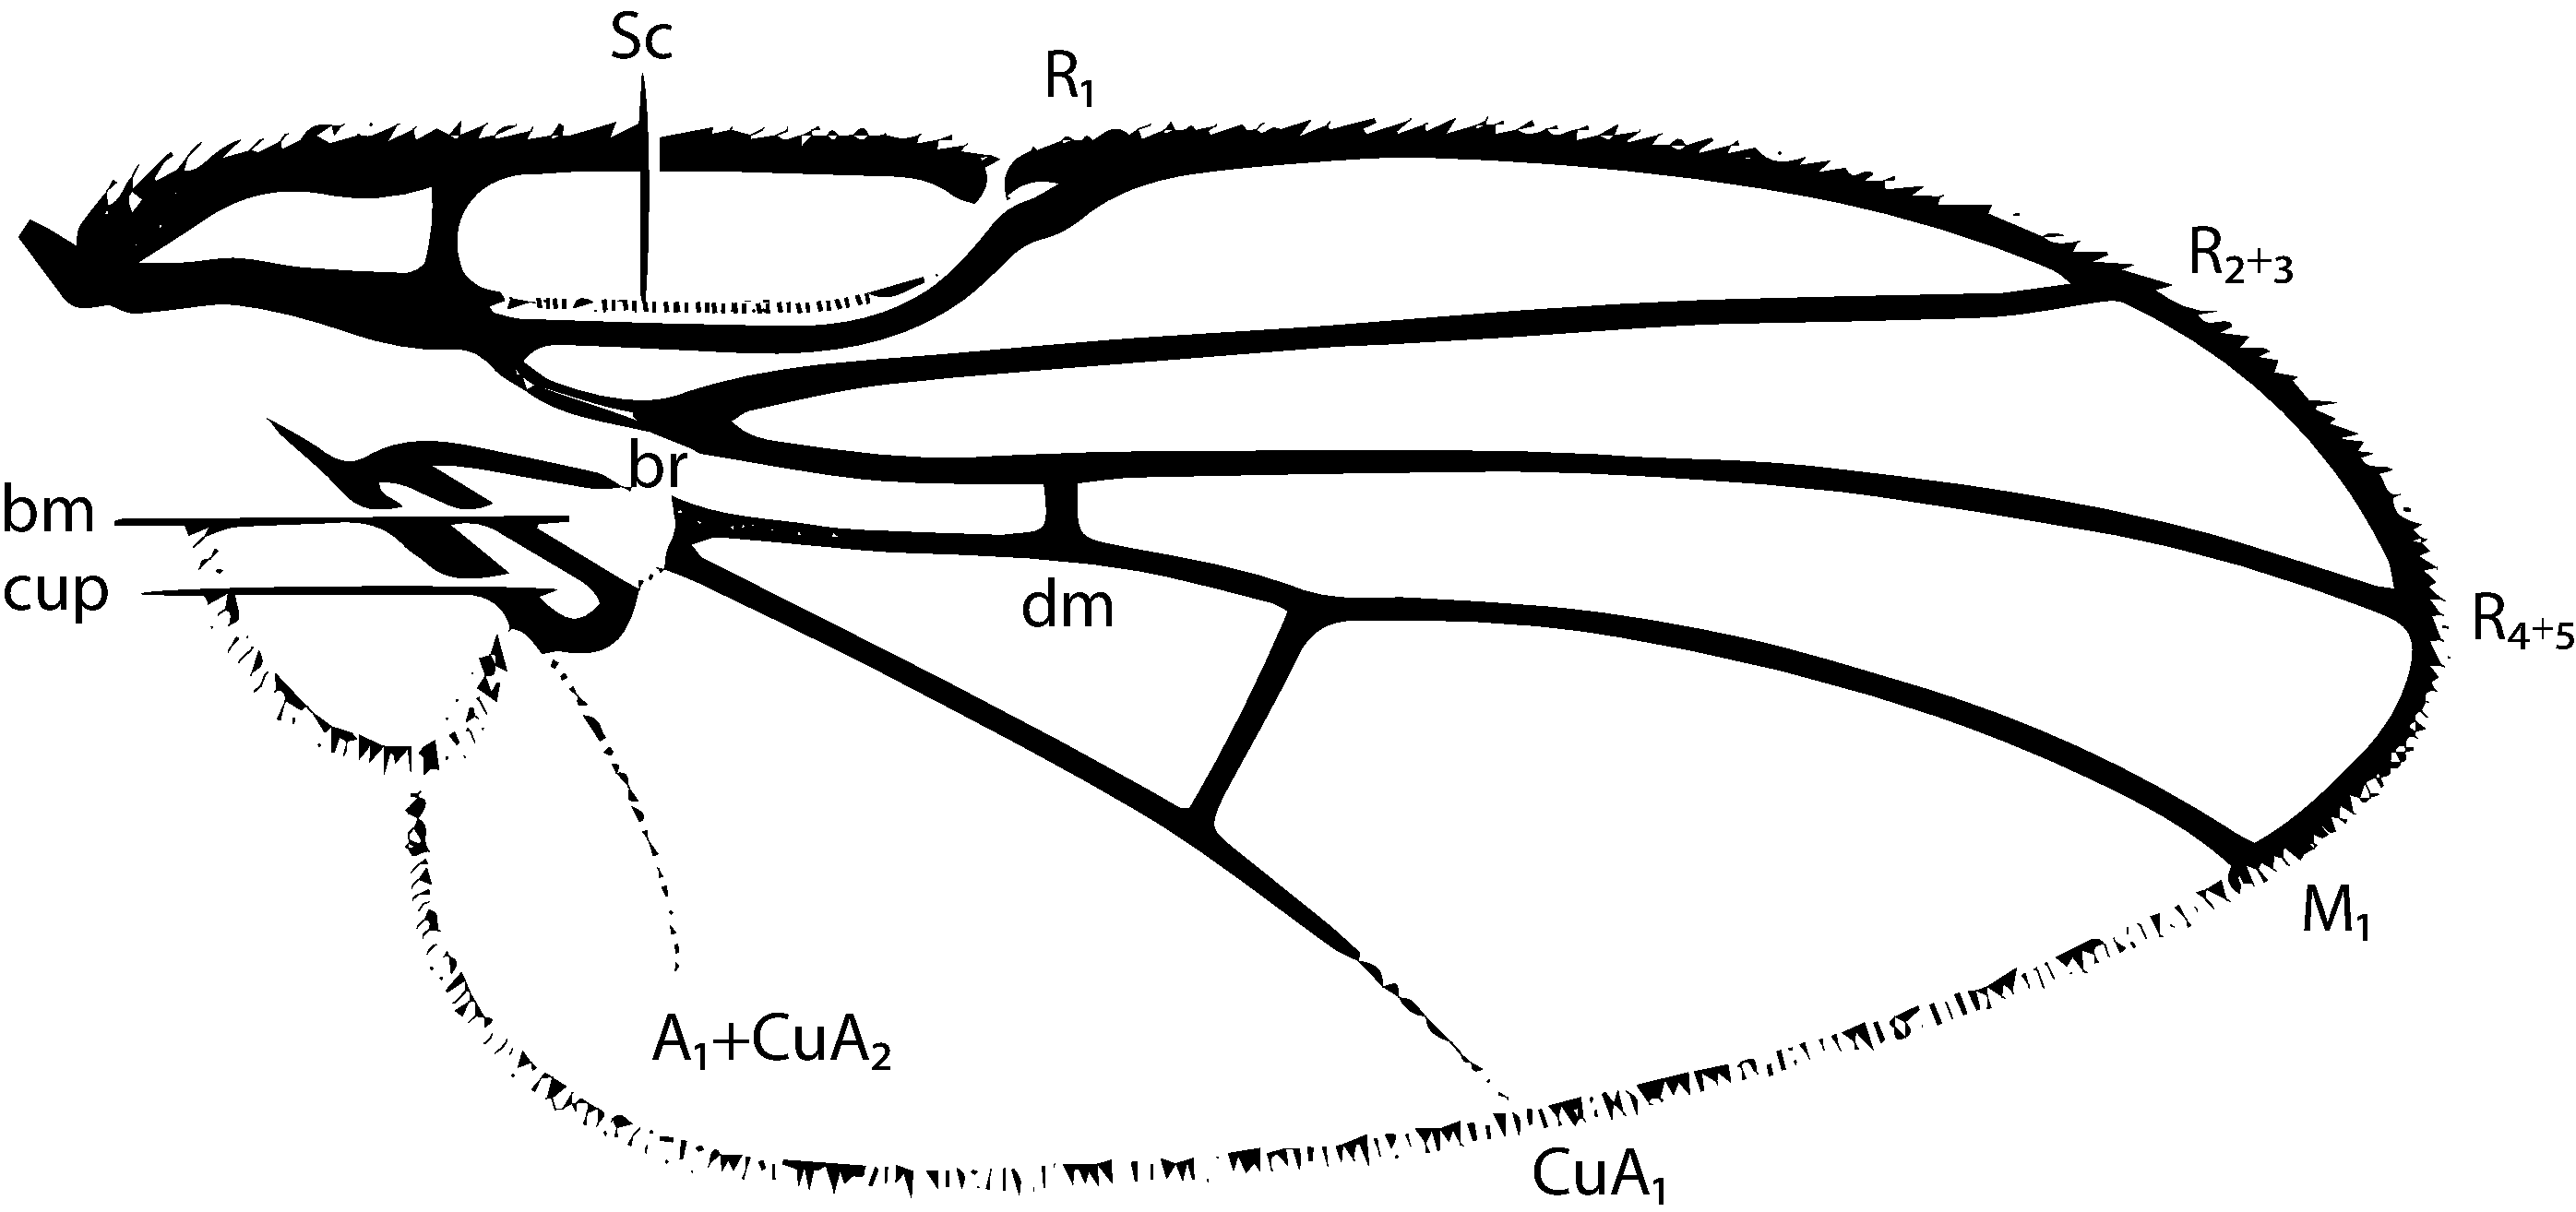
\includegraphics[width=\textwidth]{antliophora/AgromyzidWing}
        \caption{}
        \label{fig:agromyzid1}
    \end{subfigure}
    \qquad
    \begin{subfigure}[ht!]{0.3\textwidth}
        \includegraphics[width=\textwidth]{antliophora/AgromyzidHead}
        \caption{}
        \label{fig:agromyzid2}
    \end{subfigure}
    \caption{Agromyzidae. \textbf{(a)} Fore wing \citep[][Fig. 73.9]{mcalpine1981manualv2}; \textbf{(b)} head \citep[][Fig. 73.2]{mcalpine1981manualv2}}\label{fig:agromyzids}
\end{figure}

\subsubsection{Chloropidae (grass or frit flies)}\index{Chloropidae}
\noindent{}\textit{Diagnostic characters:} Sc incomplete, Costa broken once; anal cell absent; ocellar triangle greatly enlarged, usually shiny; oral vibrissae absent; diverse head shapes, smooth, very few setae; tiny, often colorful flies.\vspace{3mm}

\noindent{}\textit{Natural history:} Chloropids are difficult to characterize ecologically, as the larvae exhibit almost every conceivable life history strategy. Most larvae, however, develop as herbivores on grasses. About 2,000 species have been described worldwide.

\begin{figure}[ht!]
    \centering
    \begin{subfigure}[ht!]{0.5\textwidth}
        \includegraphics[width=\textwidth]{antliophora/ChloropidWing}
        \caption{}
        \label{fig:chloropid1}
    \end{subfigure}
    \qquad
    \begin{subfigure}[ht!]{0.25\textwidth}
        \includegraphics[width=\textwidth]{antliophora/ChloropidHead}
        \caption{}
        \label{fig:chloropid2}
    \end{subfigure}
    \caption{Chloropidae. \textbf{(a)} Fore wing \citep[][Fig. 99.36]{mcalpine1981manualv2}; \textbf{(b)} head \citep[][Fig. 99.3]{mcalpine1981manualv2}}\label{fig:chloropids}
\end{figure}

\subsubsection{Drosophilidae (pomace, vinegar flies)}\index{Drosophilidae}
\noindent{}\textit{Diagnostic characters:} Sc incomplete, costa broken twice; anal cell present; postvertical bristles converging; arista plumose; oral vibrissae present; usually small, yellowish, brownish, or grayish.\vspace{3mm}

\noindent{}\textit{Natural history:} Drosophilidae, yet another ecologically diverse family, comprises some 4,000+ described species. Several species serve as important models for a variety of genetic research, and other species are important pestiferous herbivores.

\begin{figure}[ht!]
    \centering
    \begin{subfigure}[ht!]{0.5\textwidth}
        \includegraphics[width=\textwidth]{antliophora/DrosophilidWing}
        \caption{}
        \label{fig:drosophilid1}
    \end{subfigure}
    \qquad
    \begin{subfigure}[ht!]{0.27\textwidth}
        \includegraphics[width=\textwidth]{antliophora/DrosophilidHead}
        \caption{}
        \label{fig:drosophilid2}
    \end{subfigure}
    \caption{Drosophilidae. \textbf{(a)} Fore wing \citep[][Fig. 95.6]{mcalpine1981manualv2}; \textbf{(b)} head \citep[][Fig. 95.6]{mcalpine1981manualv2}}\label{fig:drosophilids}
\end{figure}

\paragraph{Calyptratae} The remaining families are part of an apparently monophyletic taxon called Calyptratae, named for the expanded calypters of the fore wing. These insects also usually have the following characters:\index{Calyptratae}
\begin{itemize}
\item transverse suture complete on thorax
\item greater ampulla (bump at base of wing, anterior to calypters) present, enlarged 
\item antennal pedicel with complete dorsal seam
\item generally larger, more setose than acalyptrates
\end{itemize}

\begin{figure}[ht!]
  \centering
    \includegraphics[width=0.9\textwidth]{antliophora/CalyptrateMorph}
  \caption{Calyptratae morphology; \textbf{ar} = arista, \textbf{mr} = meron, \textbf{npl} = notopleuron, \textbf{npl s} = notopleural seta, \textbf{sbsctl} = subscutellum, \textbf{sctl} = scutellum \citep[][Fig. 2.66]{mcalpine1981manual}}
  \label{fig:calyptratemorph}
\end{figure}

\subsubsection{Muscidae (house flies and relatives)}\index{Muscidae}
\noindent{}\textit{Diagnostic characters:} Usually drab but is also variable in color and form; meron without row of bristles; no setae present on ventral surface of scutellum; fore wing \texorpdfstring{A\textsubscript{1}}{A1} short and not reaching margin; \texorpdfstring{R\textsubscript{5}}{R5} cell parallel-sided or narrowing distally.\vspace{3mm}

\noindent{}\textit{Natural history:} Larvae typically develop in decaying substrates, like dung and dead organisms. Adults are saprophages, blood-feeders, and/or predators of other insects. About 4,000 species have been described worldwide.

\begin{figure}[ht!]
    \centering
    \begin{subfigure}[ht!]{0.4\textwidth}
        \includegraphics[width=\textwidth]{antliophora/MuscidWings}
        \caption{}
        \label{fig:muscid1}
    \end{subfigure}
    \qquad
    \begin{subfigure}[ht!]{0.45\textwidth}
        \includegraphics[width=\textwidth]{antliophora/MuscidHabitus}
        \caption{}
        \label{fig:muscid2}
    \end{subfigure}
    \caption{Muscidae. (a) Fore wings \citep[][Fig. 105.22,24]{mcalpine1981manualv2}; (b) habitus \citep[][Fig. 105.1]{mcalpine1981manualv2}}\label{fig:muscids}
\end{figure}

\subsubsection{Anthomyiidae (root-maggot flies)}\index{Anthomyiidae}
\noindent{}\textit{Diagnostic characters:} Meron without row of bristles; \texorpdfstring{A\textsubscript{1}}{A1} reaching wing margin, at least as fold; \texorpdfstring{R\textsubscript{5}}{R5} cell always parallel-sided; scutellum with setae ventrally; almost always drab: black, gray, brown; thinner abdomen and lighter color than Muscidae.\vspace{3mm}

\noindent{}\textit{Natural history:} Larvae typically develop in decaying plant material, and many species are associated with roots. This family, comprised of about 2,000 described species, includes several important pests (\textit{e.g.}, some \textit{Delia} spp.).\vspace{3mm}

\begin{theo}
{}You may have noticed by now that many of the characters that separate families are quite subtle---characters that would almost be used to separate \textit{species} in other taxa. What does it mean to be a family \textit{vs}. a genus \textit{vs}. species?
\end{theo}

\begin{figure}[ht!]
    \centering
    \begin{subfigure}[ht!]{0.5\textwidth}
        \includegraphics[width=\textwidth]{antliophora/AnthomyiidWing}
        \caption{}
        \label{fig:anthomyiid1}
    \end{subfigure}
    \qquad
    \begin{subfigure}[ht!]{0.4\textwidth}
        \includegraphics[width=\textwidth]{antliophora/AnthomyiidThorax}
        \caption{}
        \label{fig:anthomyiid2}
    \end{subfigure}
    \caption{Anthomyiidae. \textbf{(a)} Fore wing \citep[][Fig. 104.29]{mcalpine1981manualv2}; \textbf{(b)} thorax \citep[][Fig. 104.18]{mcalpine1981manualv2}}\label{fig:anthomyiids}
\end{figure}

\subsubsection{Tachinidae (parasitic flies)}\index{Tachinidae}
\noindent{}\textit{Diagnostic characters:} Subscutellum developed (sbsctl in figure \ref{fig:calyptratemorph}); \texorpdfstring{R\textsubscript{5}}{R5} cell narrowed or closed distally; arista usually not plumose (figure \ref{fig:tachinid1}); meron with row of bristles (see figure \ref{fig:calyptratemorph}, near hind coxa (cx 3)).\vspace{3mm}

\noindent{}\textit{Natural history:} Tachinids develop as parasitoids of other invertebrates, especially insects, and most are suspected to not be very host-specific. There are well over 8,000 described species.

\begin{figure}[ht!]
    \centering
    \begin{subfigure}[ht!]{0.5\textwidth}
        \includegraphics[width=\textwidth]{antliophora/TachinidWing}
        \caption{}
        \label{fig:tachinid1}
    \end{subfigure}
    \qquad
    \begin{subfigure}[ht!]{0.21\textwidth}
        \includegraphics[width=\textwidth]{antliophora/TachinidHead}
        \caption{}
        \label{fig:tachinid2}
    \end{subfigure}
    \caption{Tachinidae. \textbf{(a)} Fore wing \citep[][Fig. 110.201]{mcalpine1981manualv2}; \textbf{(b)} head in lateral view \citep[][Fig. 110.91]{mcalpine1981manualv2}}\label{fig:tachinids}
\end{figure}

\subsubsection{Calliphoridae (blow flies)}\index{Calliphoridae}
\noindent{}\textit{Diagnostic characters:} Often (but not always!) metallic in color; arista plumose; meron with row of bristles; 2 notopleural bristles present; \texorpdfstring{R\textsubscript{5}}{R5} cell narrowed or closed distally.\vspace{3mm}

\noindent{}\textit{Natural history:} Larvae develop on carrion and dung, while adults are frequently found on flowers. Approximately 1,100 species have been described, and the family is suspected to be polyphyletic.\vspace{3mm}

\begin{figure}[ht!]
    \centering
    \begin{subfigure}[ht!]{0.5\textwidth}
        \includegraphics[width=\textwidth]{antliophora/CalliphoridWing}
        \caption{}
        \label{fig:calliphorid1}
    \end{subfigure}
    \qquad
    \begin{subfigure}[ht!]{0.3\textwidth}
        \includegraphics[width=\textwidth]{antliophora/CalliphoridHead}
        \caption{}
        \label{fig:calliphorid2}
    \end{subfigure}
    \caption{Calliphoridae. \textbf{(a)} Fore wing \citep[][Fig. 106.6]{mcalpine1981manualv2}; \textbf{(b)} head in dorsal view \citep[][Fig. 106.18]{mcalpine1981manualv2}}\label{fig:calliphorids}
\end{figure}

\subsubsection{Sarcophagidae (flesh flies)}\index{Sarcophagidae}
\noindent{}\textit{Diagnostic characters:} Not metallic, generally thorax with black/gray stripes, apex of abdomen usually reddish or orange; arista usually plumose only on proximal half (figure \ref{fig:sarcoph2}); meron with row of bristles; usually 4 notopleural bristles present, rarely 3; \texorpdfstring{R\textsubscript{5}}{R5} cell narrowed or closed distally.\vspace{3mm}

\noindent{}\textit{Natural history:} About 2,500 species have been described, and the maggots generally feed on carrion, on pollen stores of bees, or develop as parasitoids of other insects. 

\begin{figure}[ht!]
    \centering
    \begin{subfigure}[ht!]{0.5\textwidth}
        \includegraphics[width=\textwidth]{antliophora/SarcophagidWing}
        \caption{}
        \label{fig:sarcoph1}
    \end{subfigure}
    \qquad
    \begin{subfigure}[ht!]{0.25\textwidth}
        \includegraphics[width=\textwidth]{antliophora/SarcophagidHead}
        \caption{}
        \label{fig:sarcoph2}
    \end{subfigure}
    \caption{Sarcophagidae. \textbf{(a)} Fore wing \citep[][Fig. 116.30]{mcalpine1981manualv2}; \textbf{(b)} Head in antero-lateral view \citep[][Fig. 116.13]{mcalpine1981manualv2}}\label{fig:sarcophs}
\end{figure}

\subsubsection{Hippoboscidae (louse flies)}\index{Hippoboscidae}
\noindent{}\textit{Diagnostic characters:} Highly modified, louse-like in shape, often wingless; body setae relatively short; eyes often very small; coxae widely separated; venation reduced, Rs located anteriorad of typical position in Diptera; wings sometimes dehiscent (wings fell off of specimen); segmentation on abdomen indistinct.\vspace{3mm}

\noindent{}\textit{Natural history:} Adults are parasites of mammals, feeding on blood and occasionally being a nuisance. The larval stage almost reaches maturity inside the mother, who nourishes the maggot with a nutritious ``milk''. When the maggot emerges from the female it immediately pupates inside a puparium.\vspace{3mm}

\begin{figure}[ht!]
    \centering
    \begin{subfigure}[ht!]{0.5\textwidth}
        \includegraphics[width=\textwidth]{antliophora/HippoboscidHabitus}
        \caption{}
        \label{fig:hippoboscid1}
    \end{subfigure}
    \qquad
    \begin{subfigure}[ht!]{0.35\textwidth}
        \includegraphics[width=\textwidth]{antliophora/HippoboscidFemale}
        \caption{}
        \label{fig:hippoboscid2}
    \end{subfigure}
    \caption{Hippoboscidae. \textbf{(a)} Winged female \citep[][Fig. 111.1]{mcalpine1981manualv2}; \textbf{(b)} wingless female \citep[][Fig. 111.36]{mcalpine1981manualv2}}\label{fig:hippoboscids}
\end{figure}

\begin{theo}
{}How is the developmental strategy of Hipposboscidae (\textit{i.e}., laying what is essentially a pupa on the host) adaptive, given what you know about their other life history traits.
\end{theo}

\section*{Test yourself}

We discussed several traits that make flies adaptable. Why do you think are flies so diverse, relative to other orders? Can you describe the three most important traits?\vspace{3mm}

\noindent{}Diptera contains many species that arguably have the greatest impacts on human society---medical and veterinary disease vectors, agricultural pests, \textit{Drosophila}, \textit{etc}.---and yet the diversity of this order remains one of the least explored. How can you explain this paradox?

\clearpage
\thispagestyle{empty}
